\chapter{Galaxy catalog as ground truth}\label{ch:galaxy-catalog-as-ground-truth}
As discussed in the previous chapter we will use the galaxy catalog $\galcat$ as the ground truth for the EMRI detection simulation and the evaluation of the posterior probability distribution of $\rhubble$. This means we disregard the incompleteness of the galaxy catalog and assume that all galaxies that exist are in the catalog. Further, we ignore any cosmological predictions on the mass and or redshift distribution of EMRI events, i.e. $p_\text{EMRI}(z, \Mbh) = 1$. This work is meant to, on the one hand verify the parameter estimation results obtained in other works and on the other hand compare the posterior distribution, hence the constraints on the reduced Hubble constant $\rhubble$ when using the black hole mass $\Mbh$ as an additional parameter compared to just using ($\dl, \varphi, \vartheta$). The procedure is as follows:
\begin{enumerate}
    \item prepare the galaxy catalog, i.e. estimate the black hole masses via \fullref{eq:stellar-mass-bh-mass-relation}.
    \item choose a random galaxy from the catalog.
    \item use the $\dl$-$z$ relation (\fullref{eq:luminosity-distance-redshift-relation-lcdm}) to compute the luminosity distance $\dl$ of the event with $\htrue = 0.73$.
    \item generate the EMRI LISA response in the form of the TDI $A,E,T$ channels.
    \item check if SNR > $\varrho_\text{th} = 20$.
    \item collect detections with Cramér-Rao bounds.
    \item draw measured best guess parameters from gaussian distributions with the true parameters as mean and the Cramér-Rao bounds as standard deviation.
    \item compute the posterior probability distribution of $\rhubble$ for the collected set of detections.
\end{enumerate}

\section{Simulated detections}\label{sec:galaxy-catalog-only-simulated-detections}
In our simulation we have collected a total of $N_\text{det} = 1580$ detections. In \fullref{fig:SNR-distribution} we show the SNR distribution of the simulated detections and the correlation to $dl$. Note that, since we chose the simulation galaxy position from a gaussian distribution of the mean and error provided in the catalog, which can lead to galaxies that are extremely close to $\dl = 0$ and therefore produce very high SNR values. We further show the distribution of all simulated events (detected and undetected) in the $\Mz-z$ plane in \fullref{fig:total-mass-redshift-distribution}. First, the distribution follows the galaxy distribution of the galaxy catalog, as expected. Second, we see that the undetected events are distributed on the upper bound on the mass range and for increasing redshifts, while the detection fraction at low redshifts is nearly $1$ everywhere, which aligns well with \cite[Figure 10]{PhysRevD.95.103012}. One remark on the generation time of the simulated events can be made, because the only true dependents of the generation time is w.r.t. the initial inclination angle $I$, as shown in \fullref{fig:inclination-generation-time}. For the Parameter estimation we use the full set of detections $N_\text{det} = 1580$. While for the posterior distribution and constraints on $\rhubble$ we use a reduced set of detections $N_\text{det}^\text{posterior} = 223$ which we talk about in the next section.

\subsection{Reduced detections for posterior evaluation}\label{subsec:galaxy-catalog-only-reduced-detections-by-relative-luminosity-error}
For the computation of the posterior distribution we further reduce the number of used detections, because detections with large relative luminosity errors $\frac{\Delta \dl}{\dl}$ are uninformative and the final shape of the posterior is always determined by the most informative detections, i.e. those with small relative luminosity distance errors. We choose a second threshold in addition to $\varrho_\text{th} = 20$ for the relative luminosity distance error $\frac{\Delta \dl}{\dl} < 0.05$. This is common in Mock data analysis and in \cite{Gair_2023} the chosen value is for example $\frac{\Delta \dl}{\dl} = 0.1$. This reduces the number of detections to $N_\text{det}^\text{posterior} = 223$. We show the new detection distribution in the $\Mz-z$ plane in \fullref{fig:reduced-mass-redshift-distribution}.


\begin{figure}
    \centering
    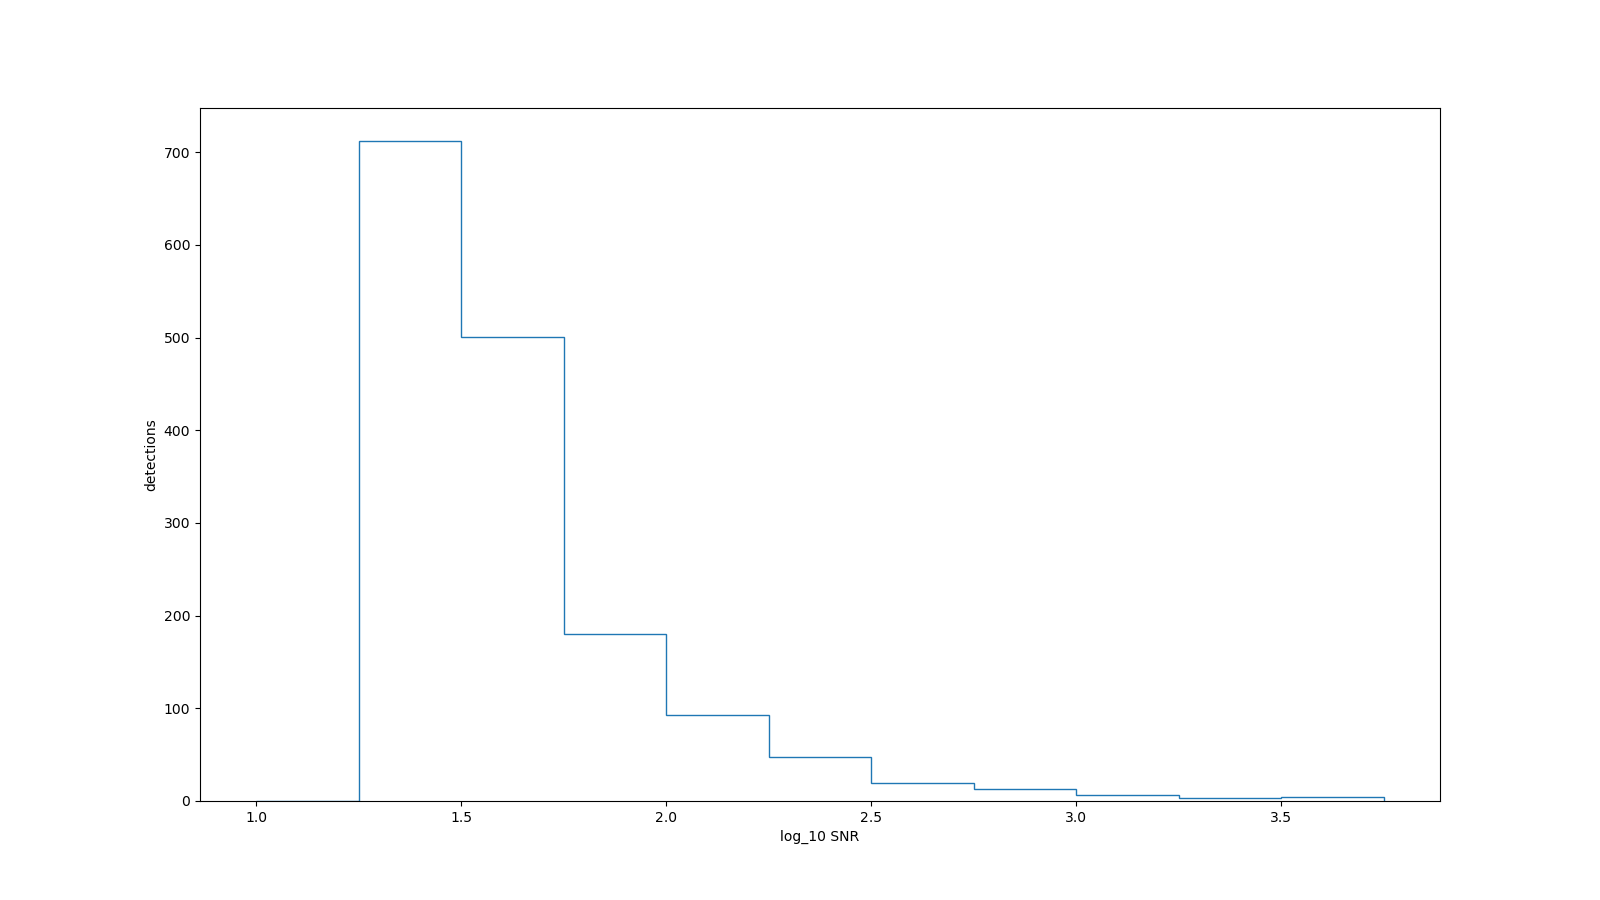
\includegraphics[width=0.49\textwidth]{simulated_detections/SNR_detections.png}
    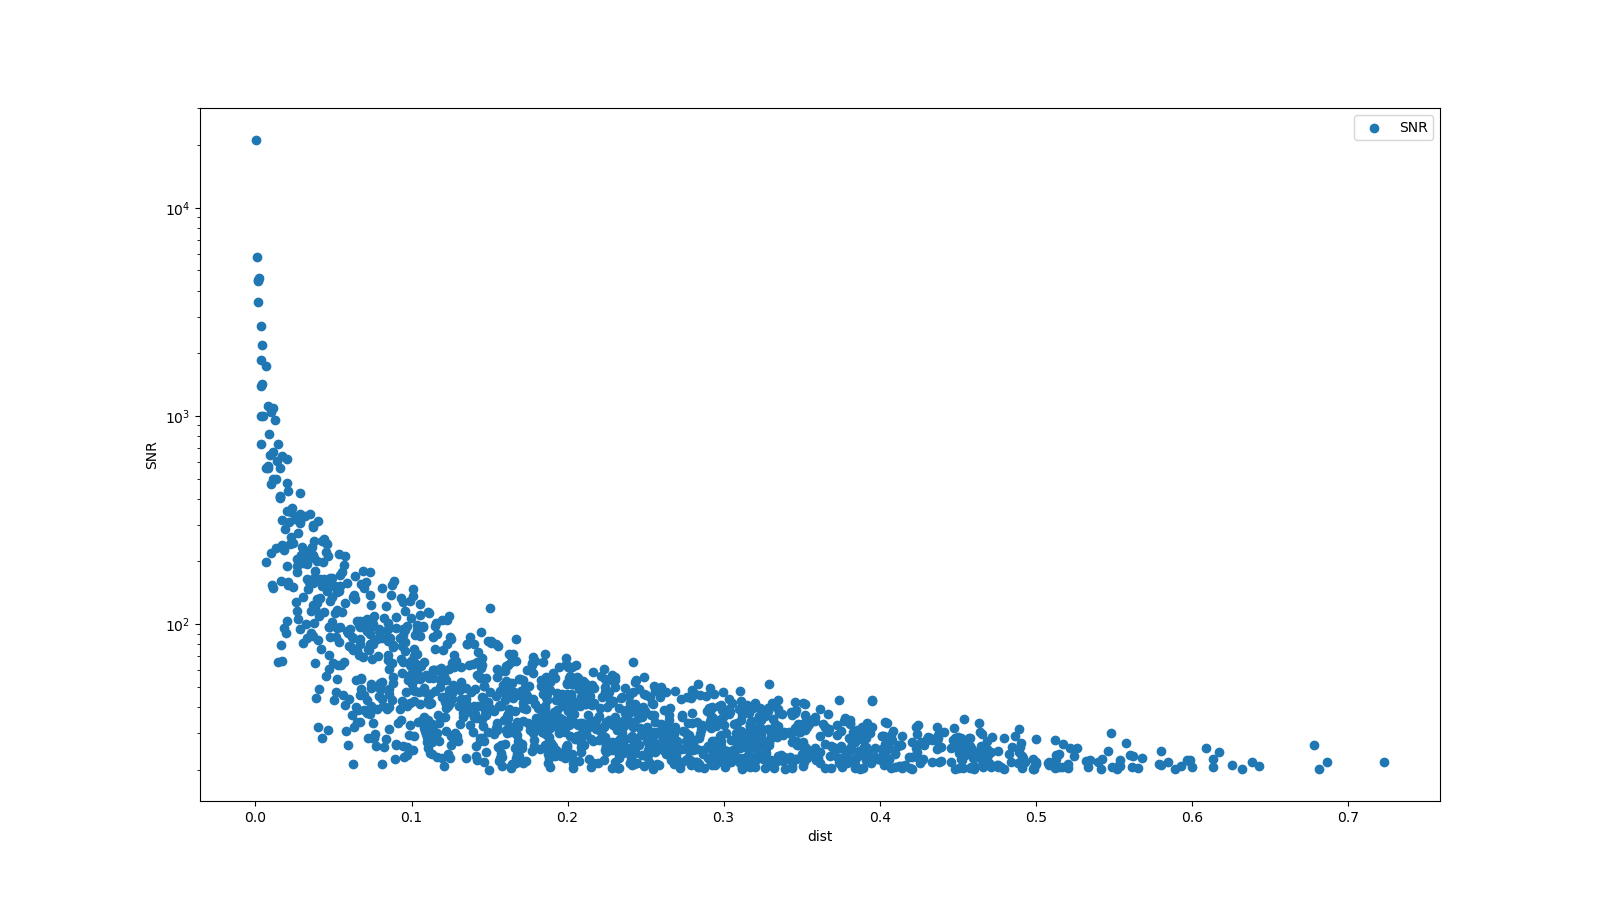
\includegraphics[width=0.49\textwidth]{simulated_detections/dist_SNR.png}
    \caption[SNR distribution of detections]{Top panel: The distribution of SNR values of the simulated detections. Bottom panel: The correlation of luminosity distance $\dl$ to the SNR of the simulated events $N_\text{det}$.}
    \label{fig:SNR-distribution}
\end{figure}

\begin{figure}
    \centering
    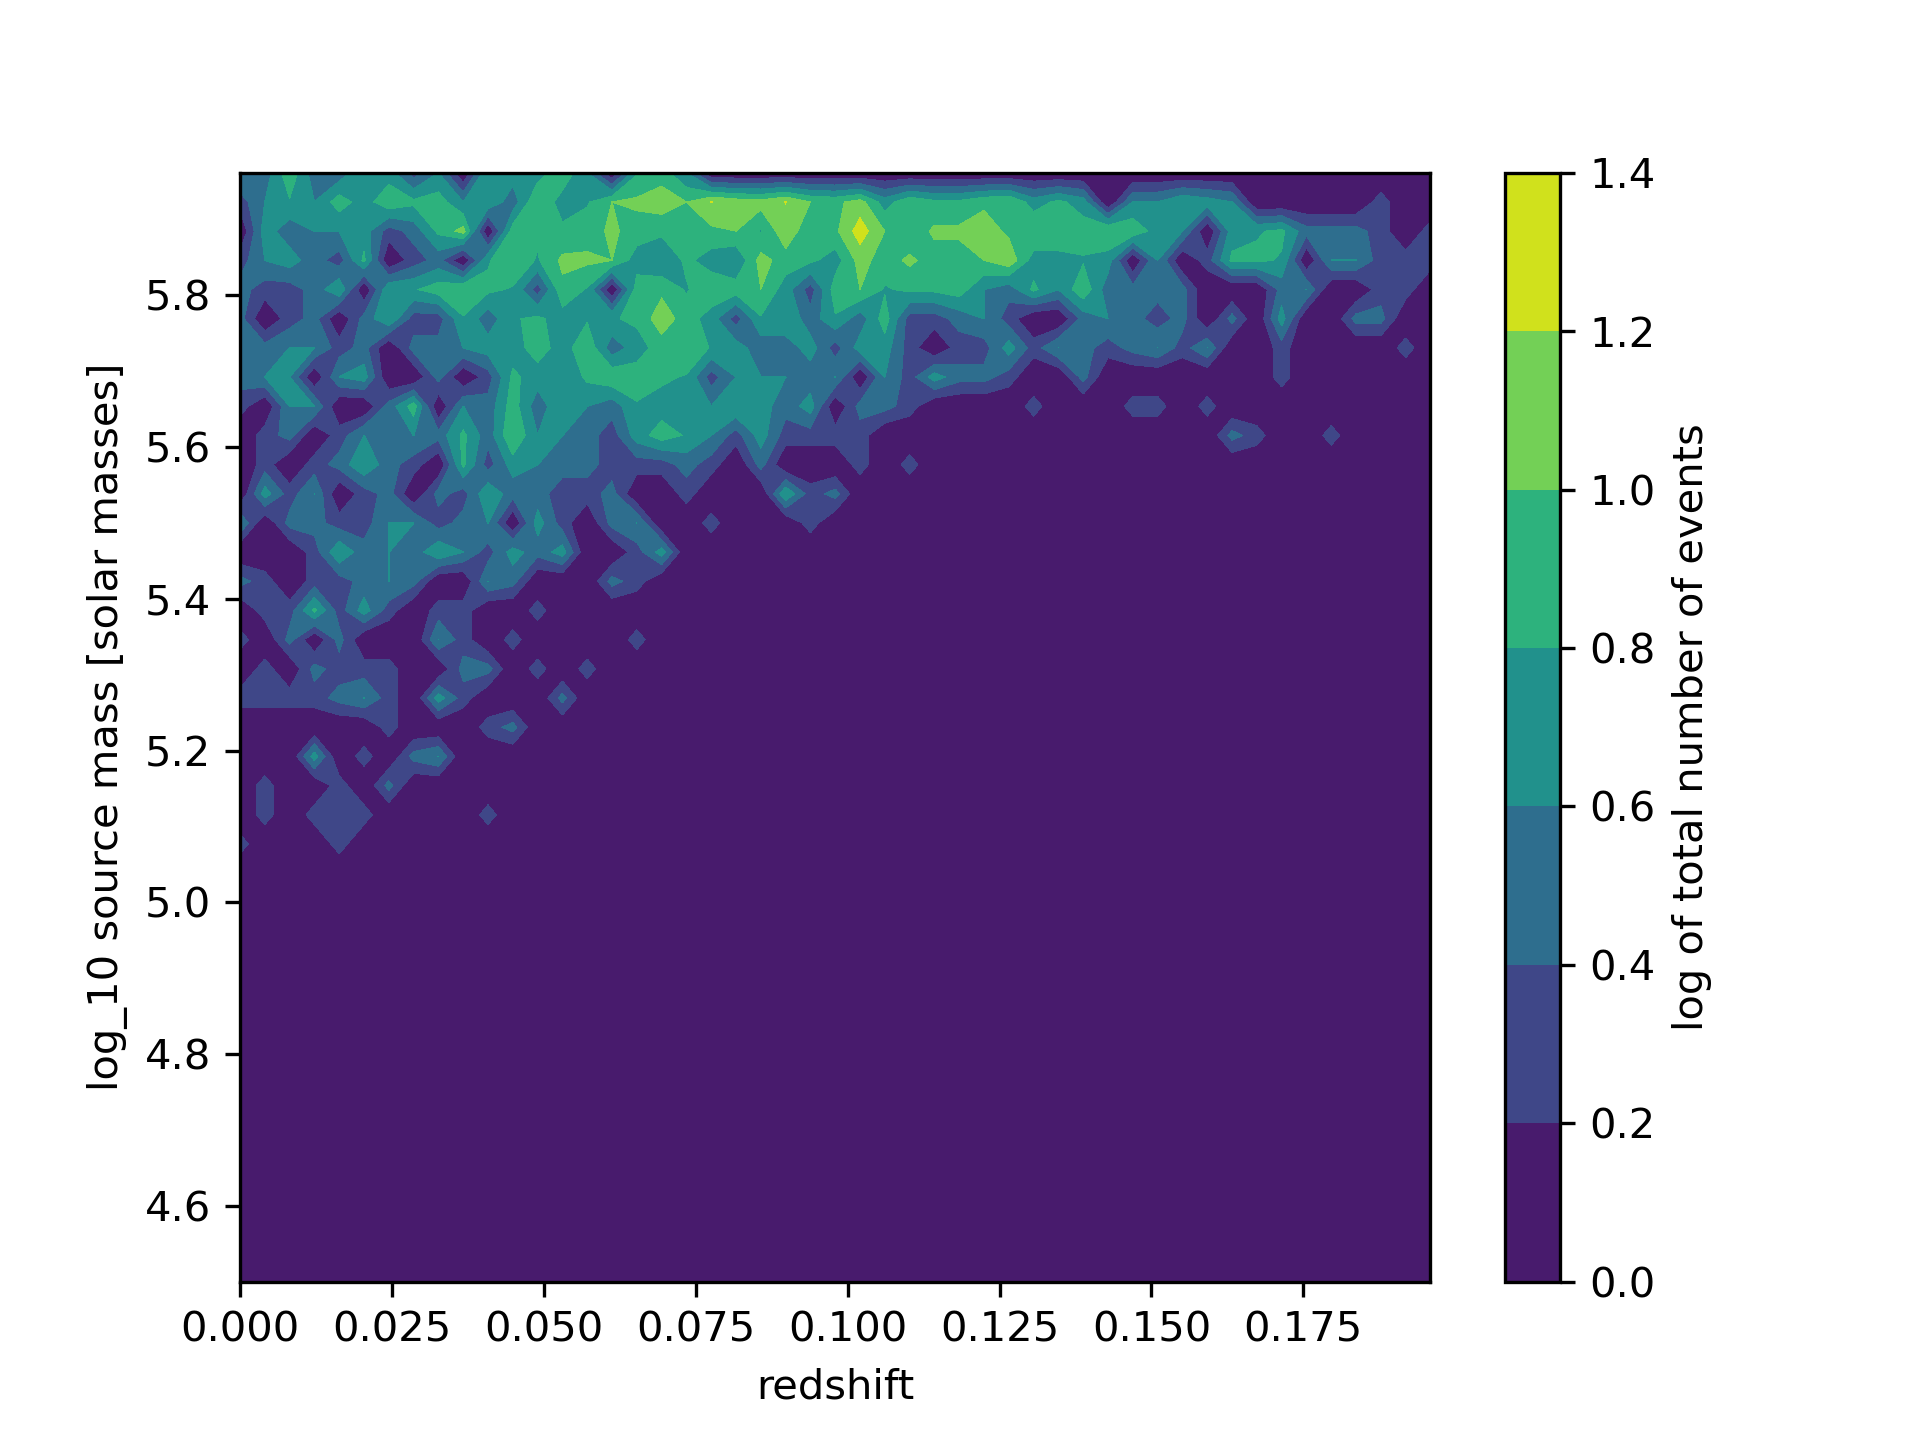
\includegraphics[width=0.49\textwidth]{simulated_detections/mass_redshift_total_number_of_events.png}
    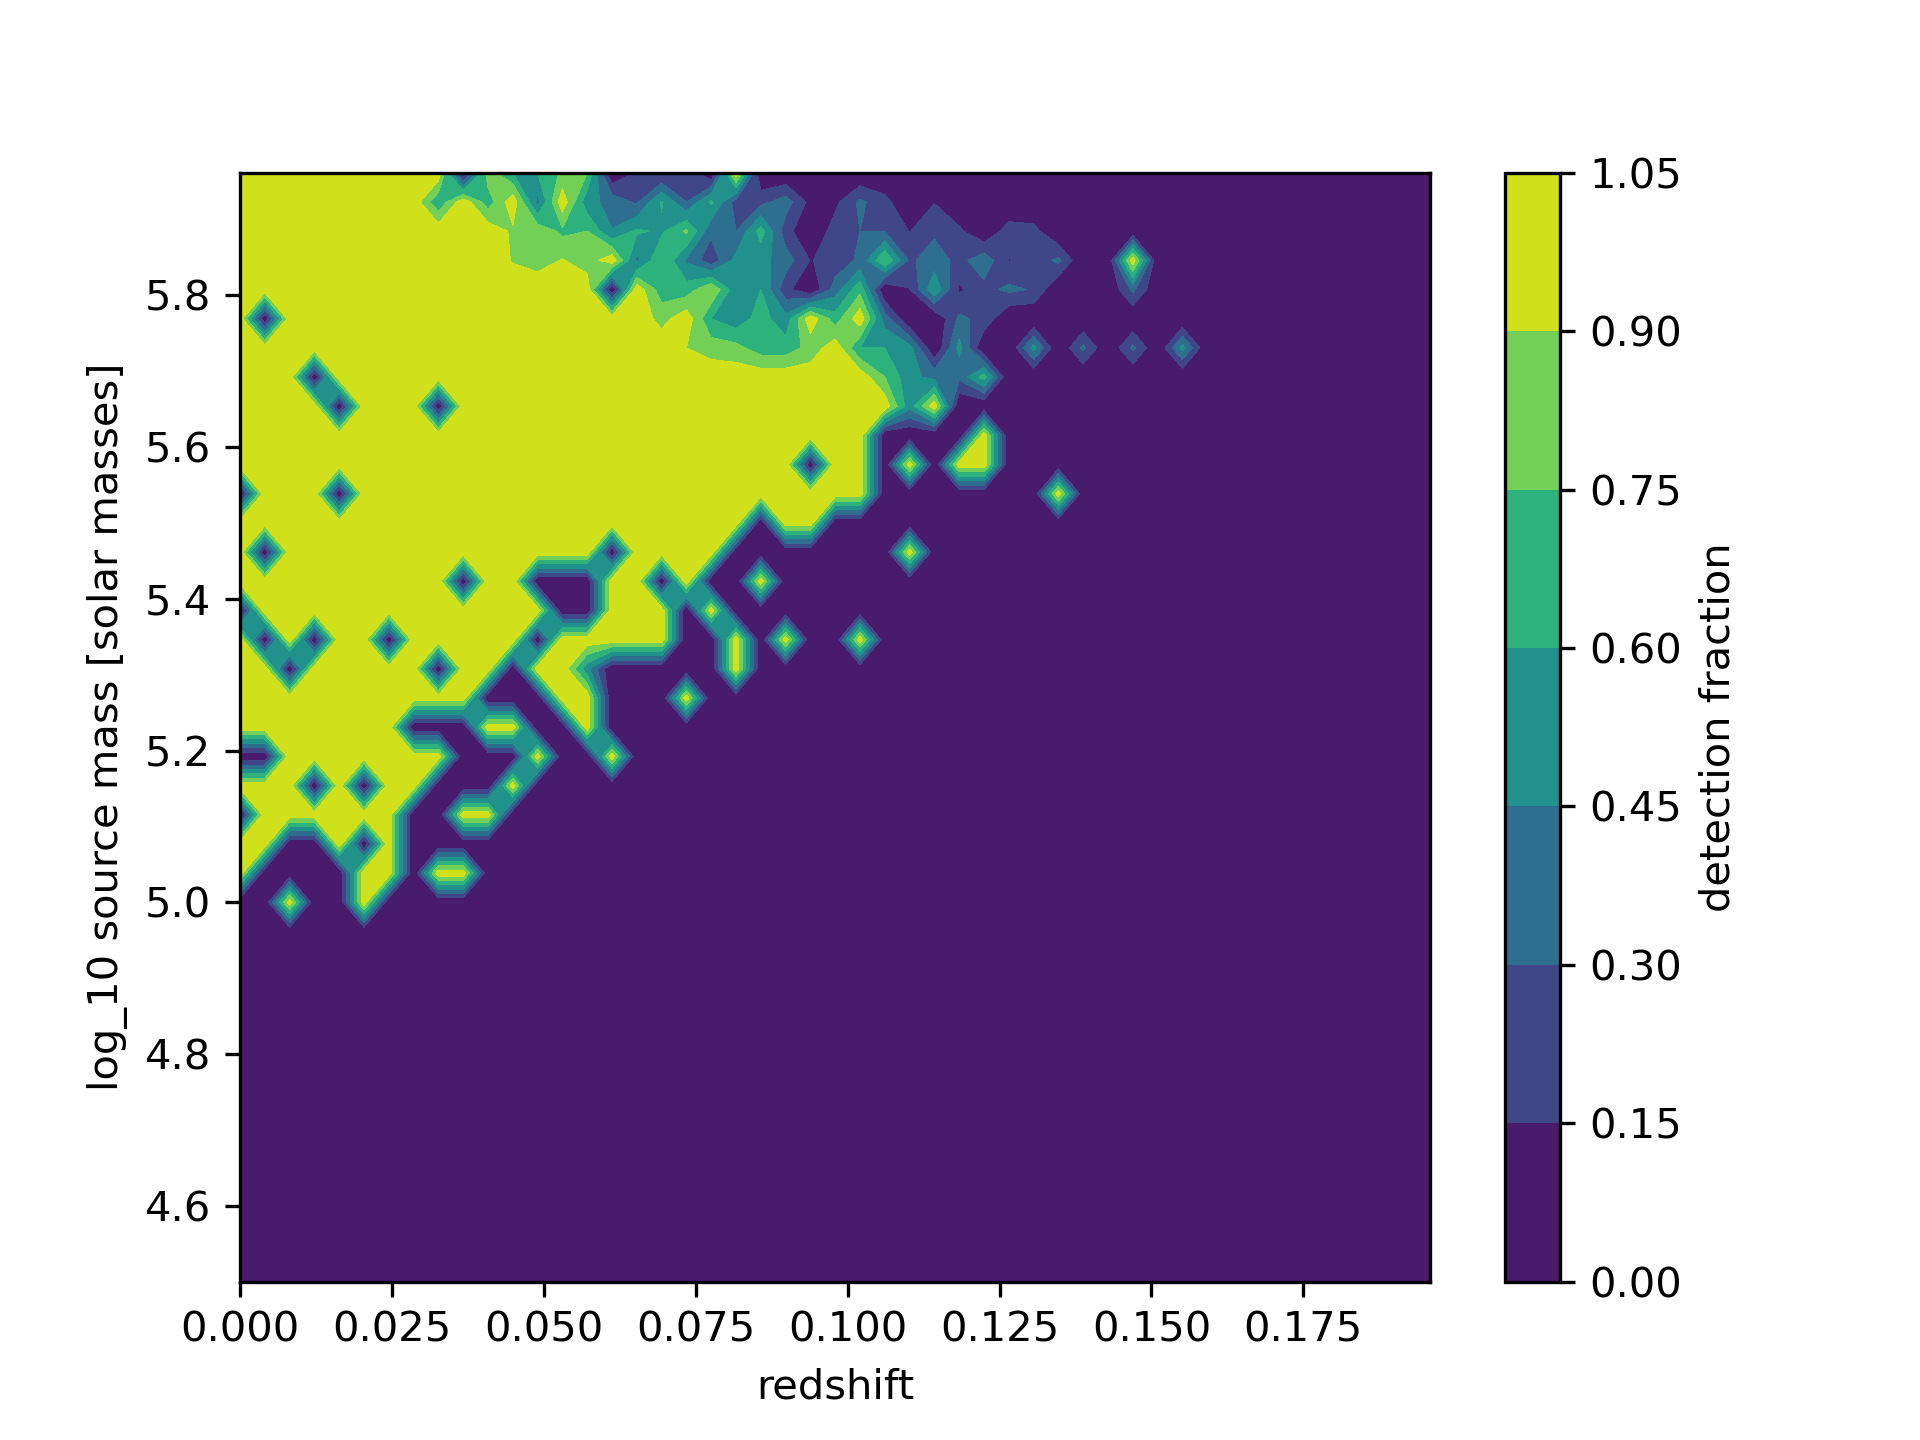
\includegraphics[width=0.49\textwidth]{simulated_detections/mass_redshift_detection_fraction.png}
    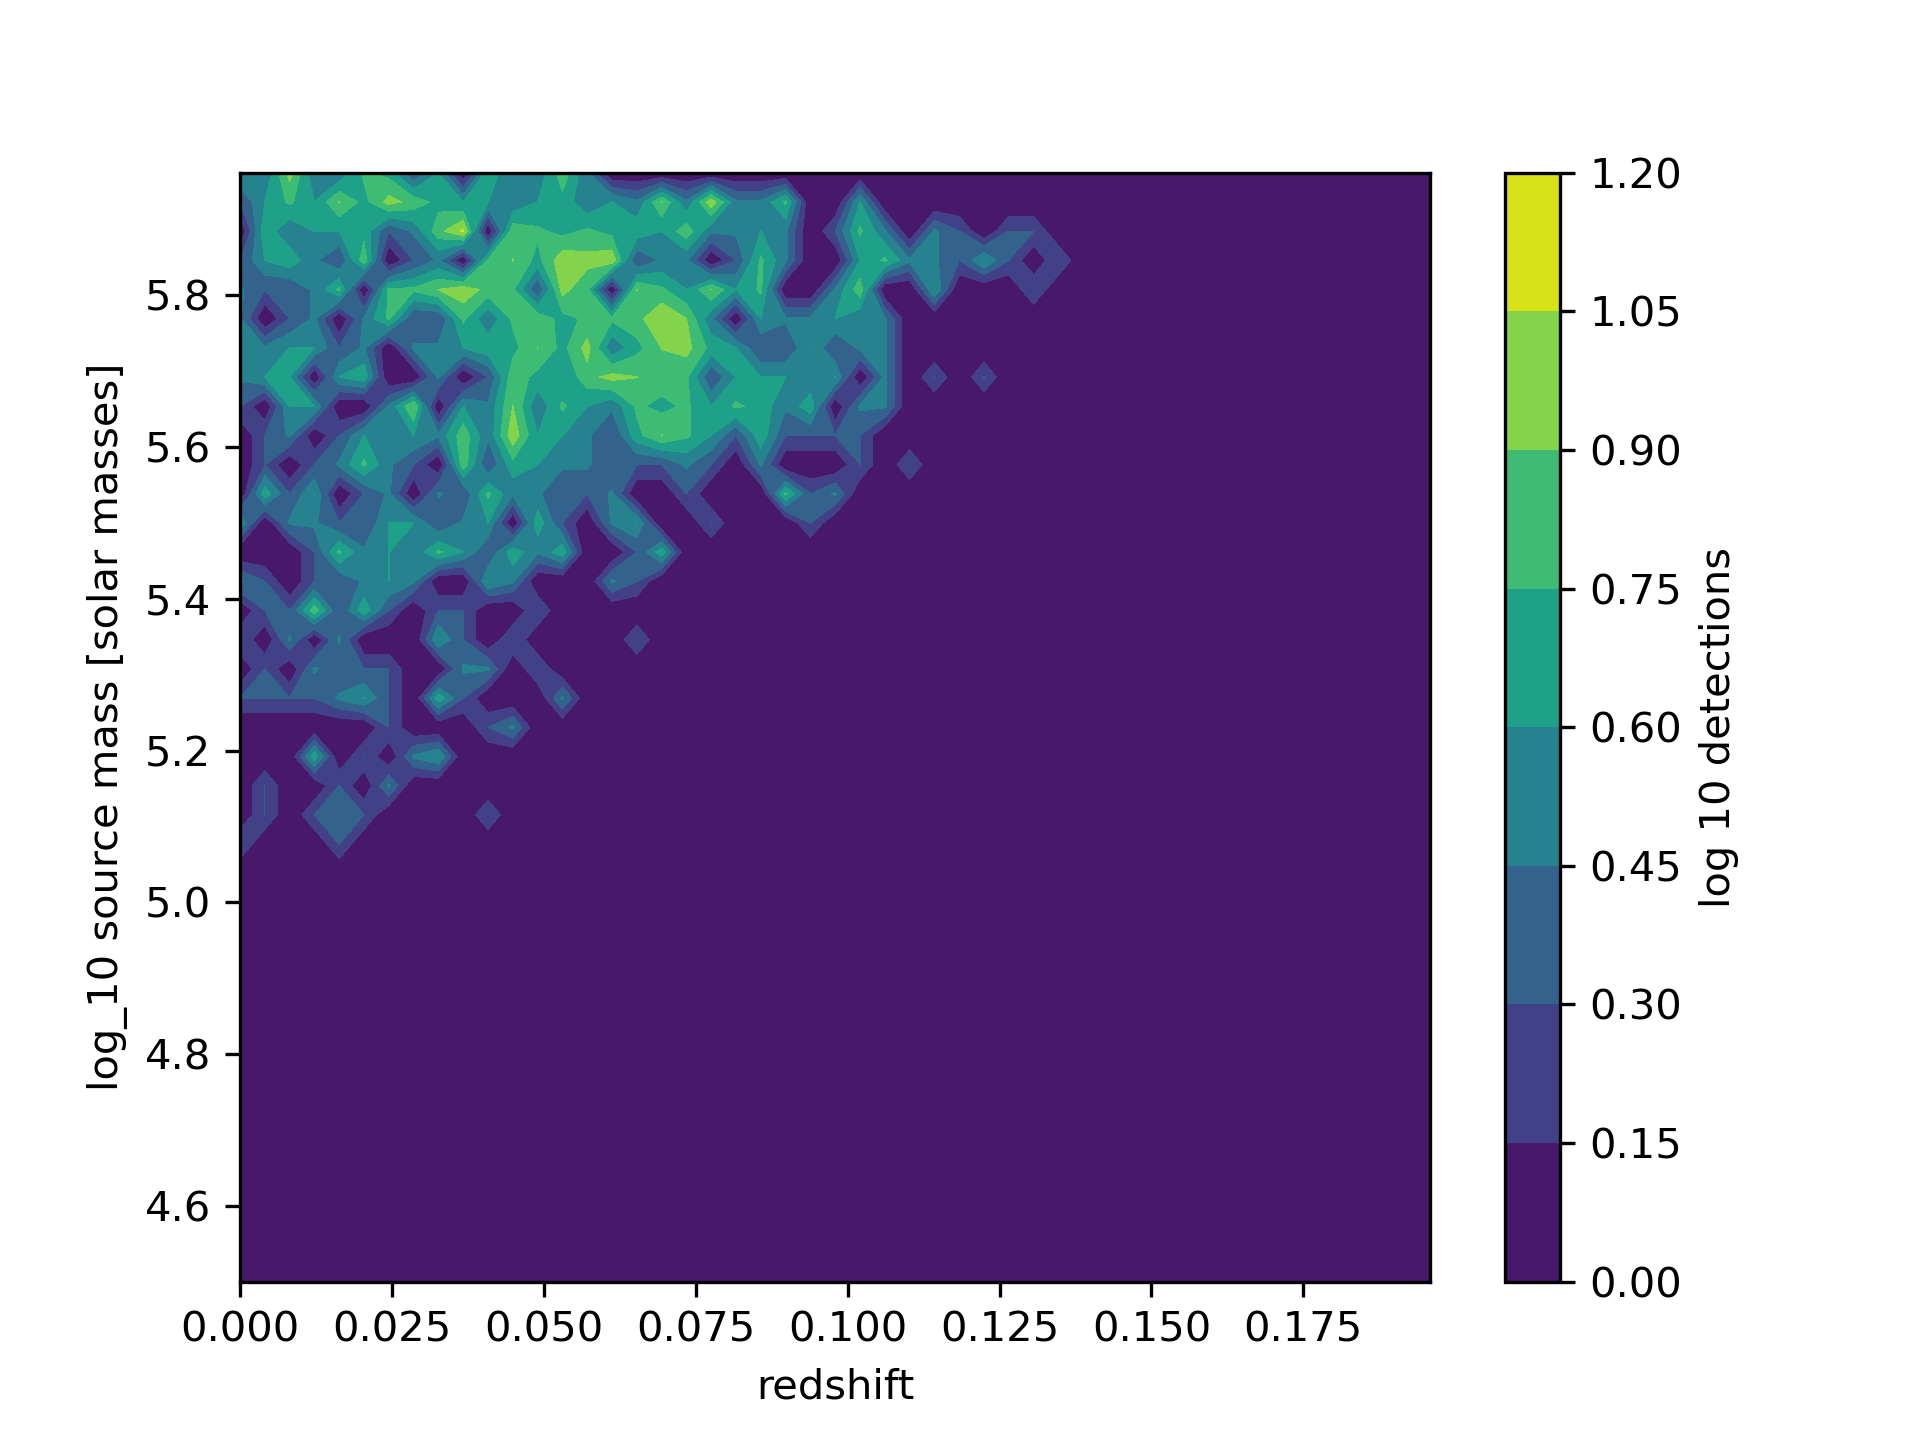
\includegraphics[width=0.49\textwidth]{simulated_detections/mass_redshift_detections.png}
    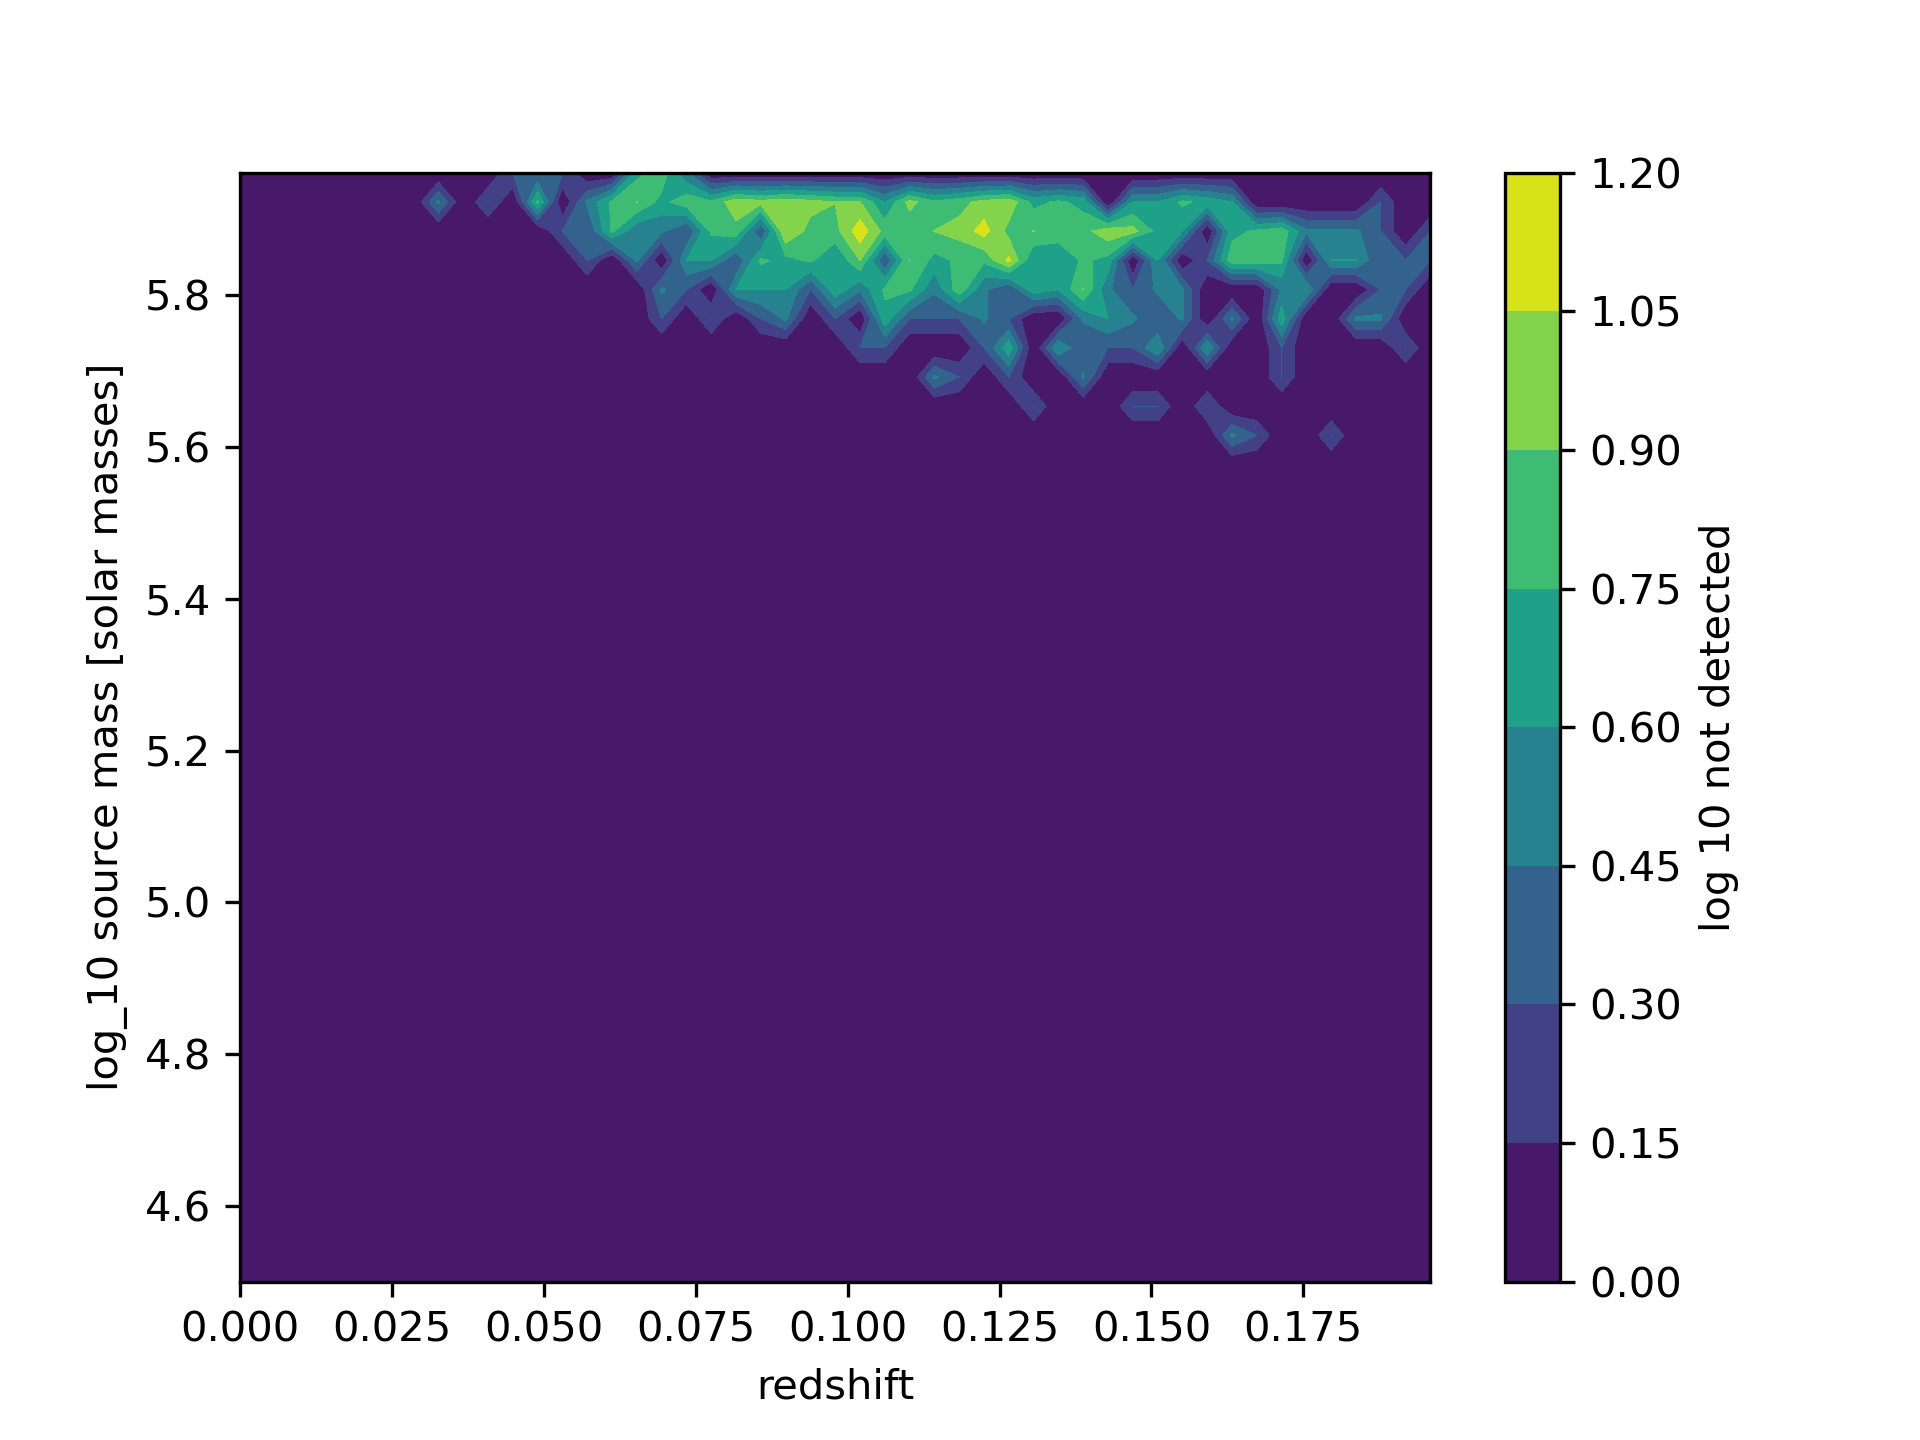
\includegraphics[width=0.49\textwidth]{simulated_detections/mass_redshift_not_detected.png}
    \caption[Mass-redshift distribution events]{Top left panel: The distribution of all simulated events in the $\Mz-z$ plane. Top right panel: The fraction of detected events in the $\Mz-z$ plane. Bottom left panel: The distribution of detected events in the $\Mz-z$ plane. Bottom right panel: The distribution of undetected events in the $\Mz-z$ plane.}
    \label{fig:total-mass-redshift-distribution}
\end{figure}
\begin{figure}
    \centering
    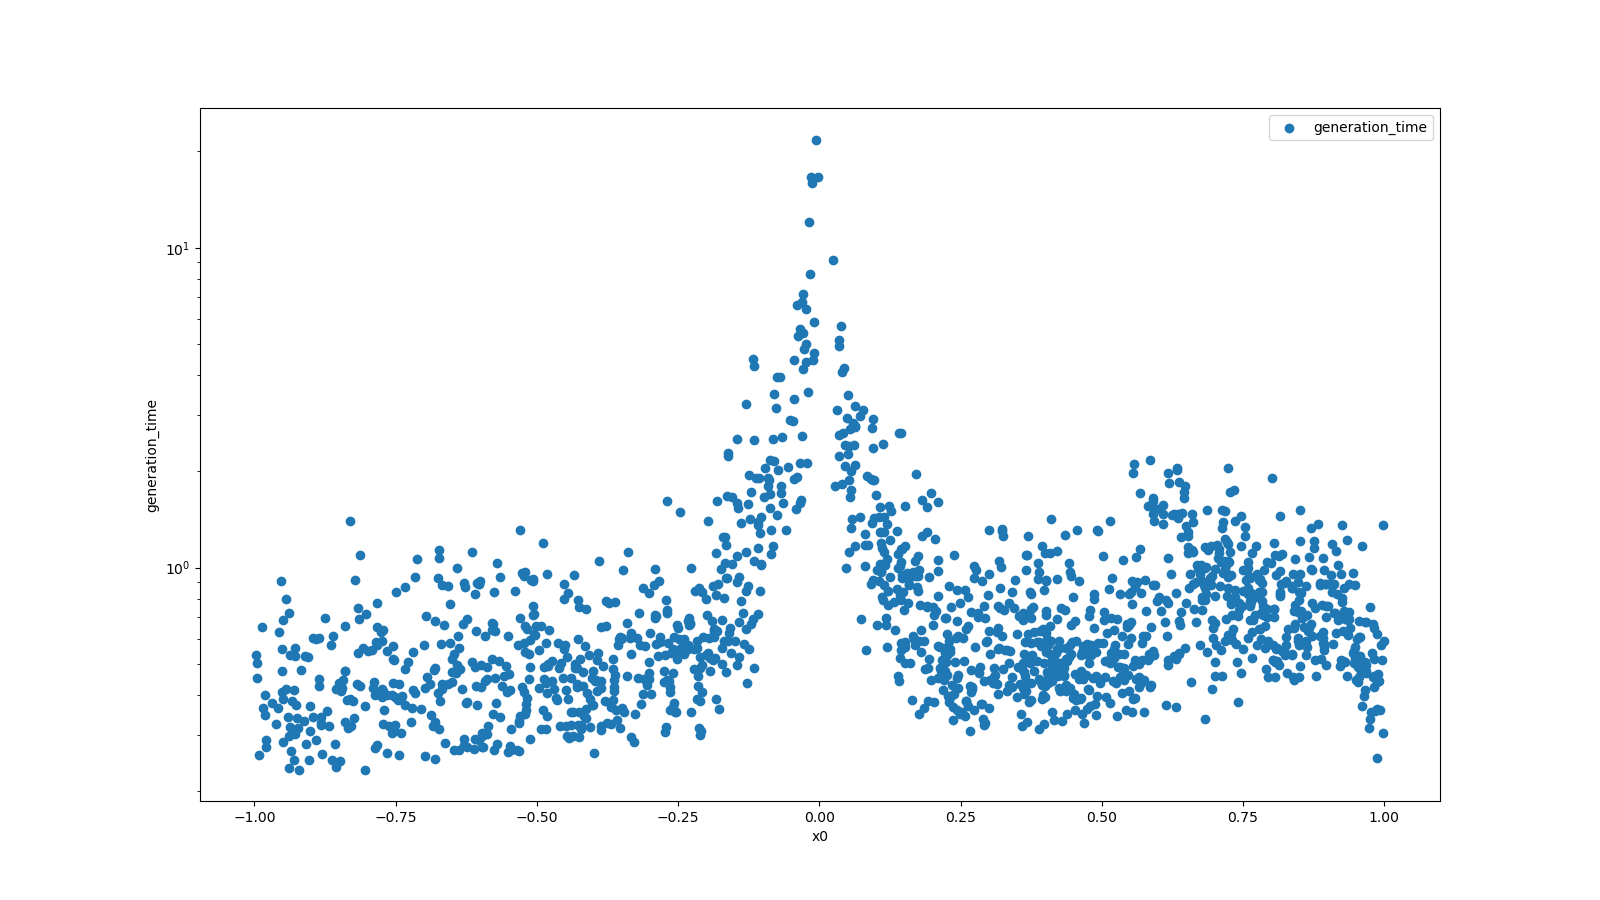
\includegraphics[width=0.8\textwidth]{simulated_detections/x0_generation_time.png}
    \caption[Inclination-generation time dependence]{Shows the the generation time of the simulated events w.r.t. the initial inclination angle $I$, i.e. $x_0 = \cos(I)$.}
    \label{fig:inclination-generation-time}
\end{figure}

\begin{figure}
    \centering

    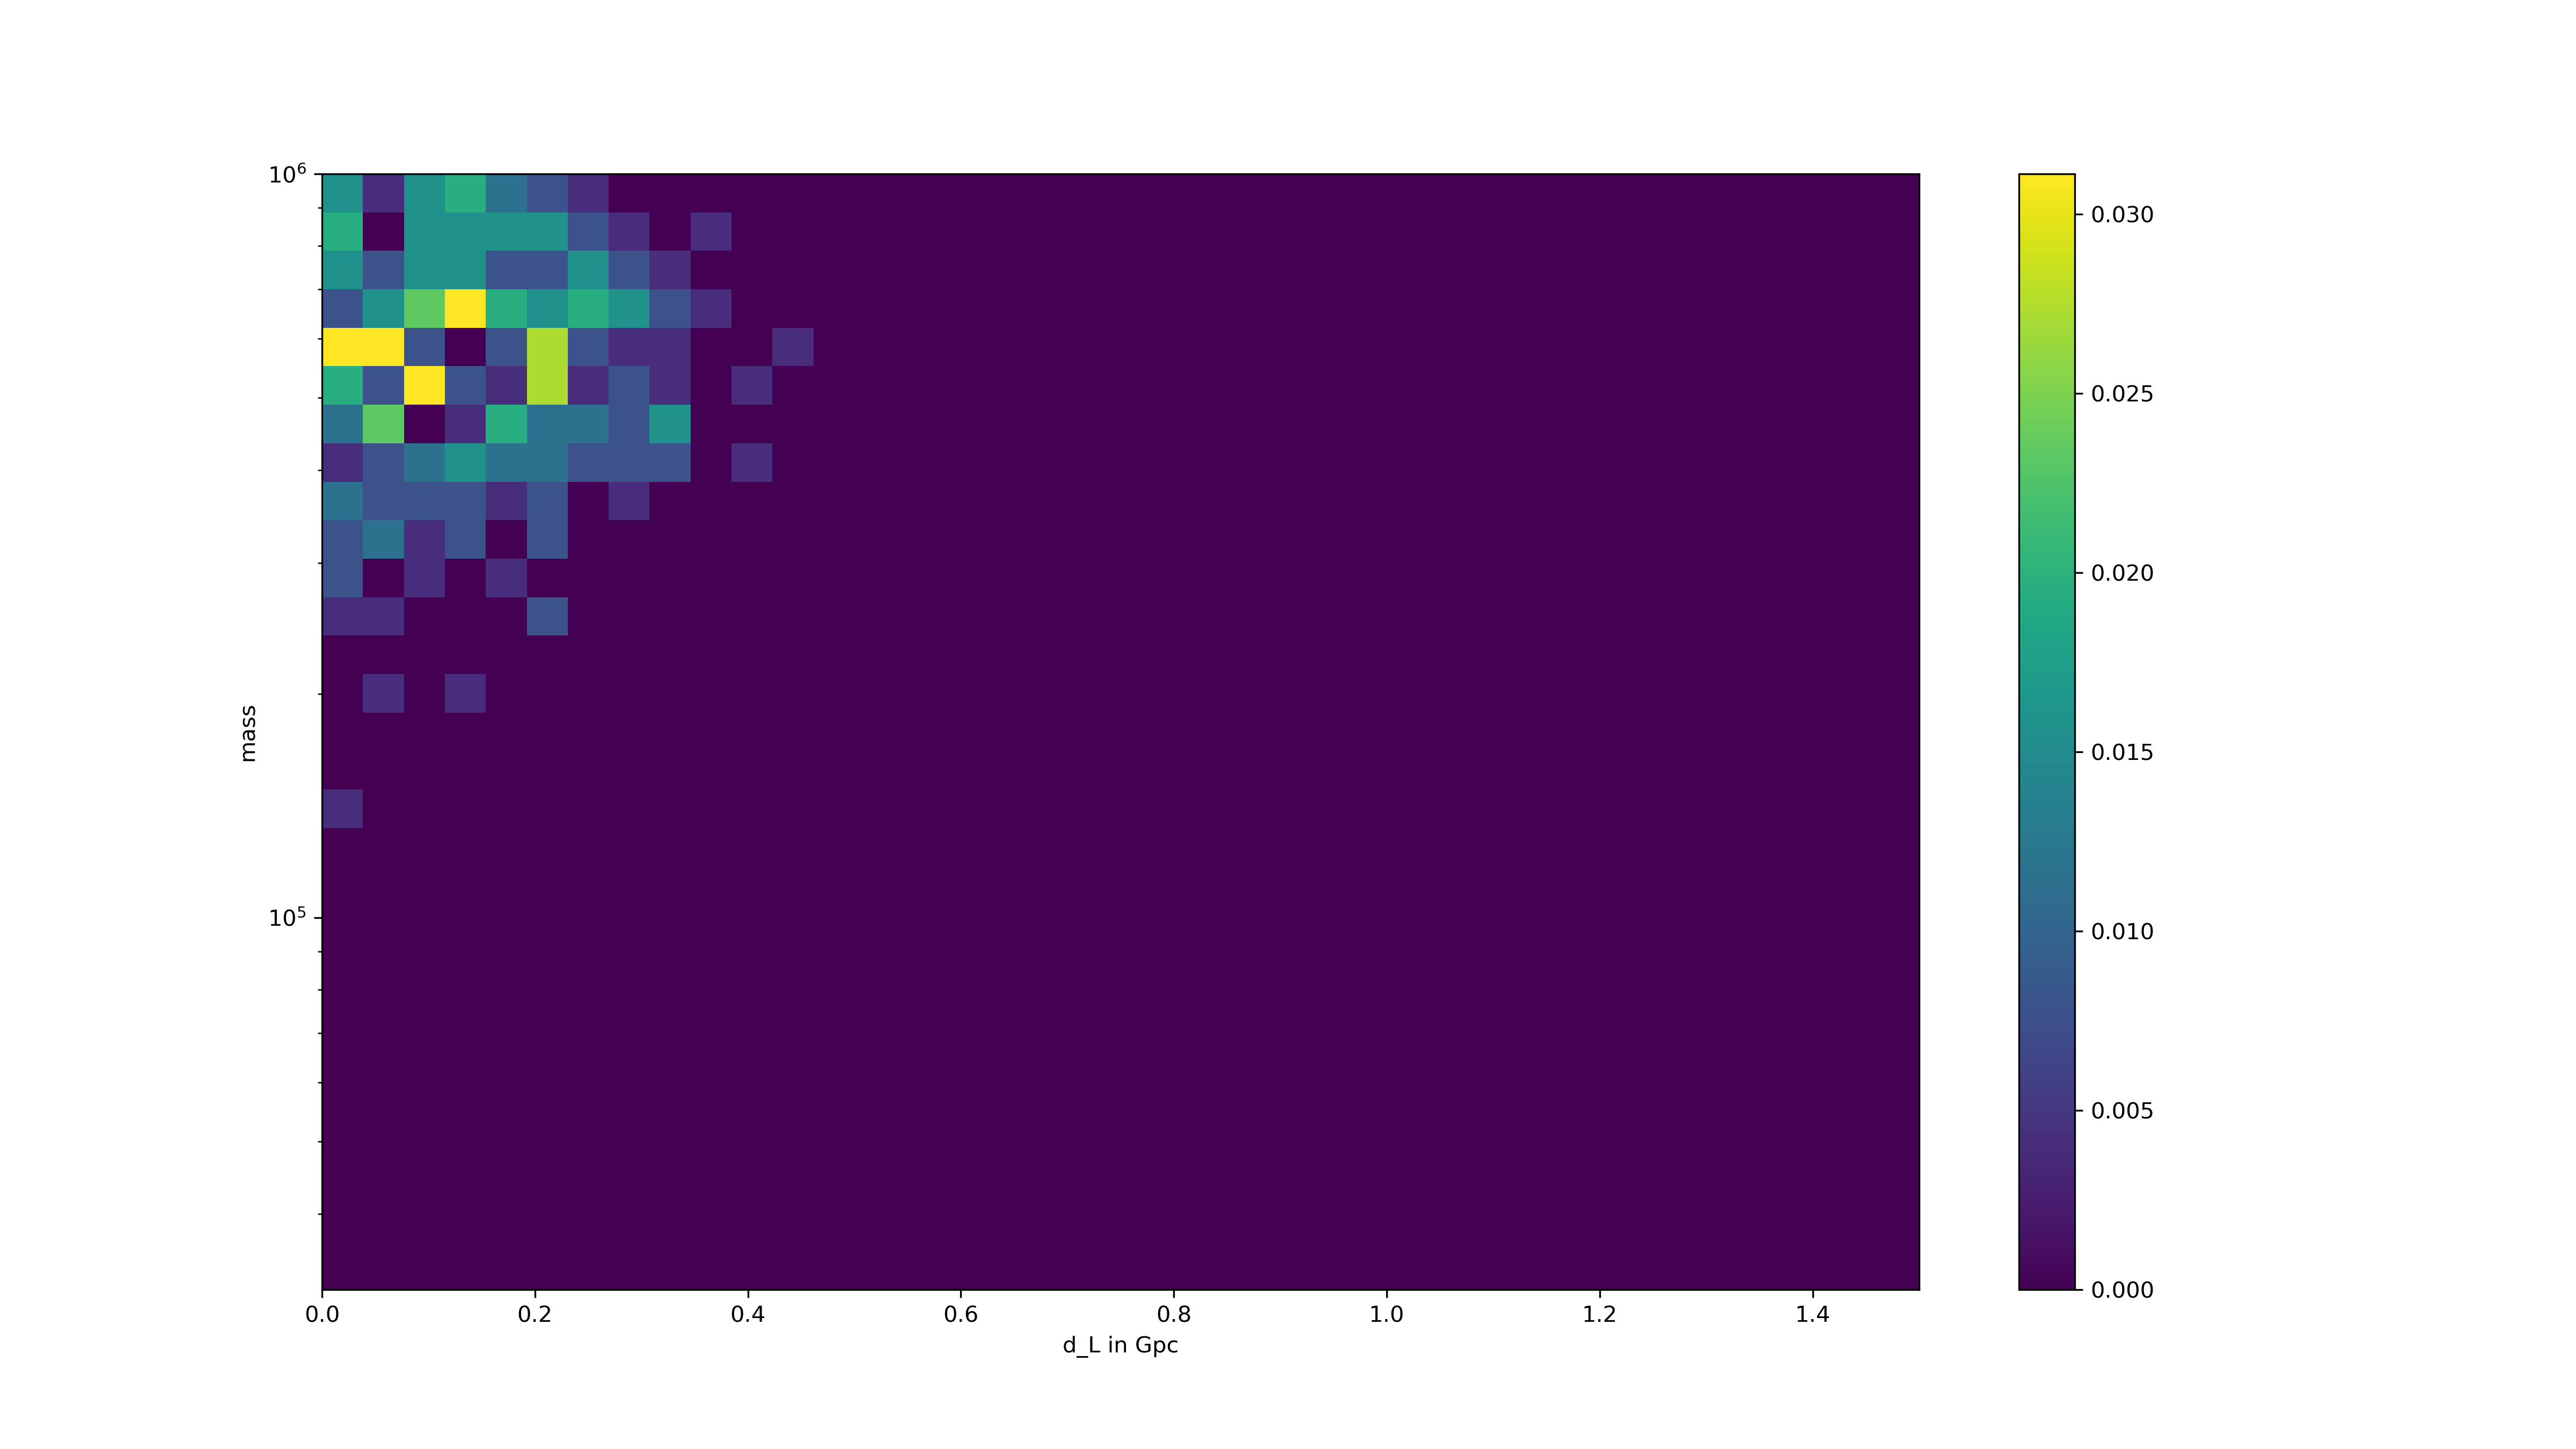
\includegraphics[width=0.8\textwidth]{simulated_detections_for_posterior/detection_hist_mass_redshift.png}
    \caption[Mass-redshift distribution for events with small relative luminosity error]{The distribution of detected events in the $\Mz-z$ plane after reducing the number of detections by imposing a threshold on the relative luminosity distance error $\frac{\Delta \dl}{\dl} = 0.05$.}
    \label{fig:reduced-mass-redshift-distribution}
\end{figure}
\section{Parameter estimation results}\label{sec:galaxy-catalog-only-parameter-estimation-results}
The parameter estimation has been derived in \fullref{sec:parameter-estimation}. To compare the results of the parameter estimation, i.e. the errors on the measured parameters by LISA to the results in \cite{PhysRevD.95.103012} we show the results for the parameters $\{ \Mz, \mu, \dl, e_0, a, (\vartheta, \varphi) \}$. For the sky localization parameters ($\vartheta, \varphi$) we compute
\begin{equation}
    \Delta \Omega \definedas 2 \pi \abs{\sin(\vartheta)} \sqrt{\sigma_{\vartheta}^2 \sigma_{\varphi}^2 - \text{cov}(\vartheta, \varphi)^2},
\end{equation}
where $\Delta \Omega$ is the probability $1-\exp\{ -1 \}$ of containing the source, called the \emph{sky localization error}. We show the results in \fullref{fig:parameter-estimation-results-galaxy-catalog-only}. The results are in perfect agreement with the results in \cite{PhysRevD.95.103012}. The average relative error for $\Mz$ also shown in \fullref{fig:relative-mass-error-distribution} is even 2 orders of magnitude lower. Hence, we can conclude that the parameter estimation is working as expected with potentially even better expected measurements of the redshifted MBH mass $\Mz$ than so far expected. This should still be verified in a more realistic simulation of the EMRI events distribution since the detection distribution we collected corresponds to very low redshifts compared to the distributions obtained in \cite{PhysRevD.95.103012}.


\begin{figure}
    \centering
    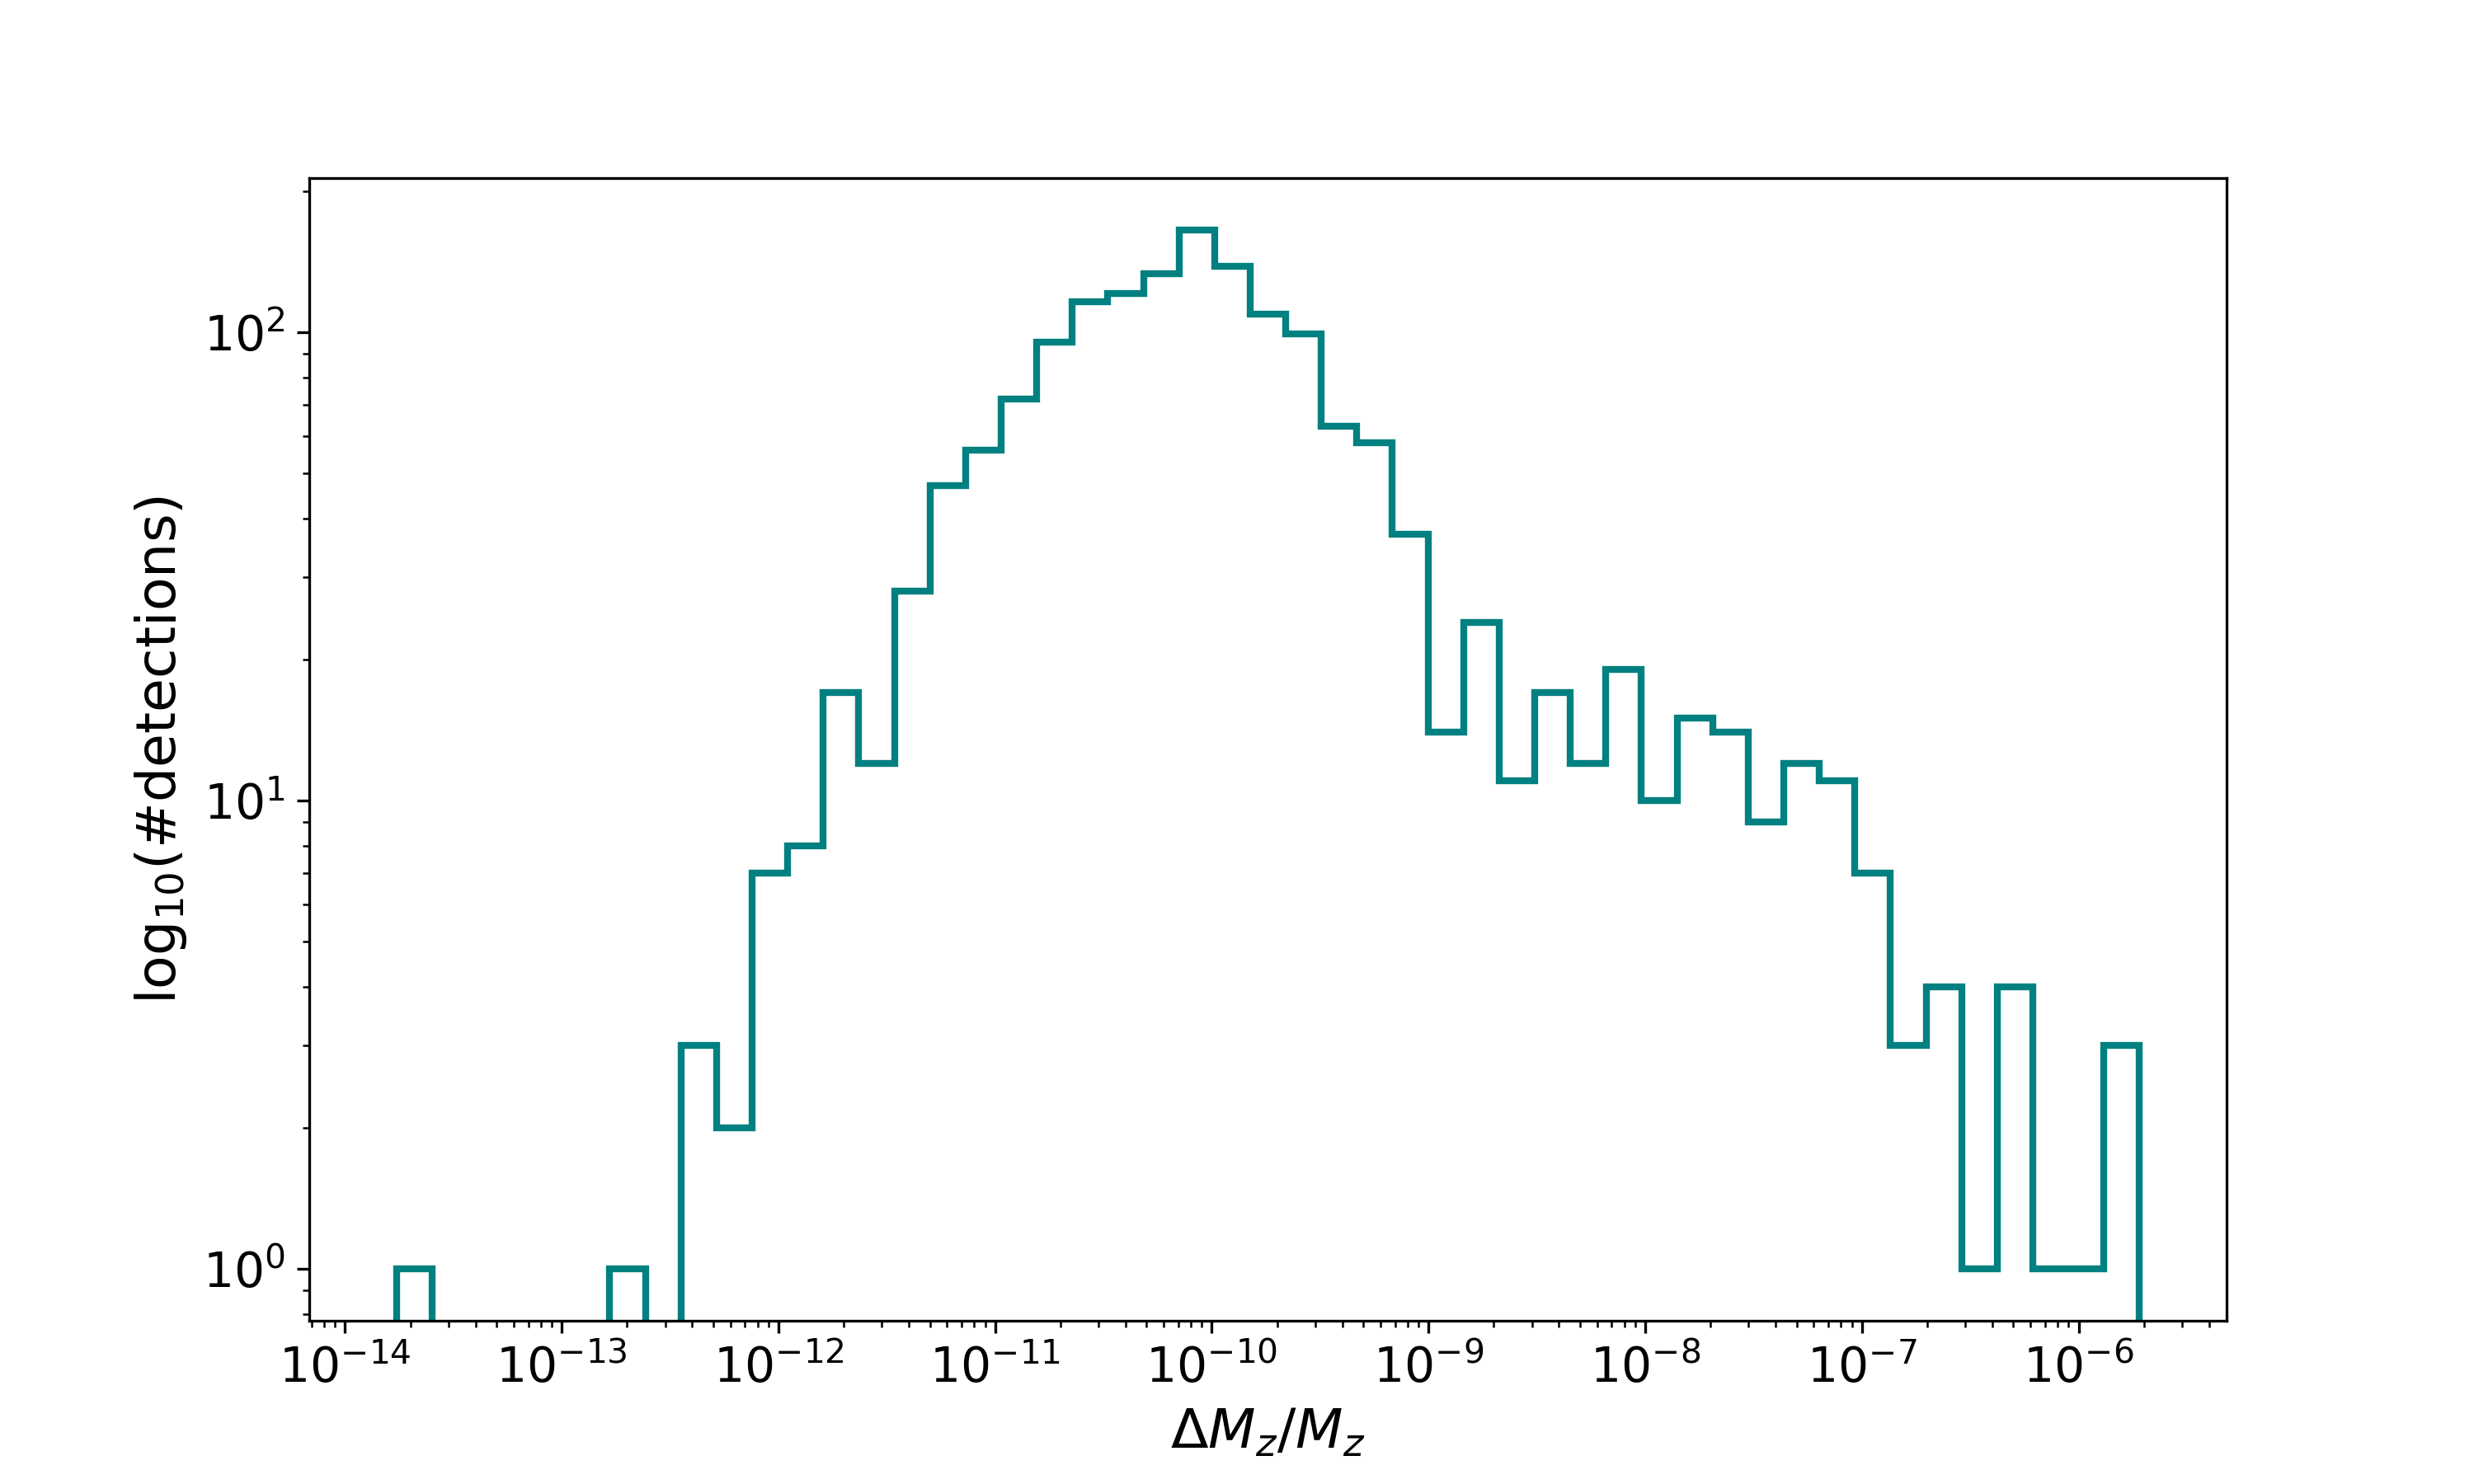
\includegraphics[width=0.49\textwidth]{parameter_estimation/mz_uncertainties.png}
    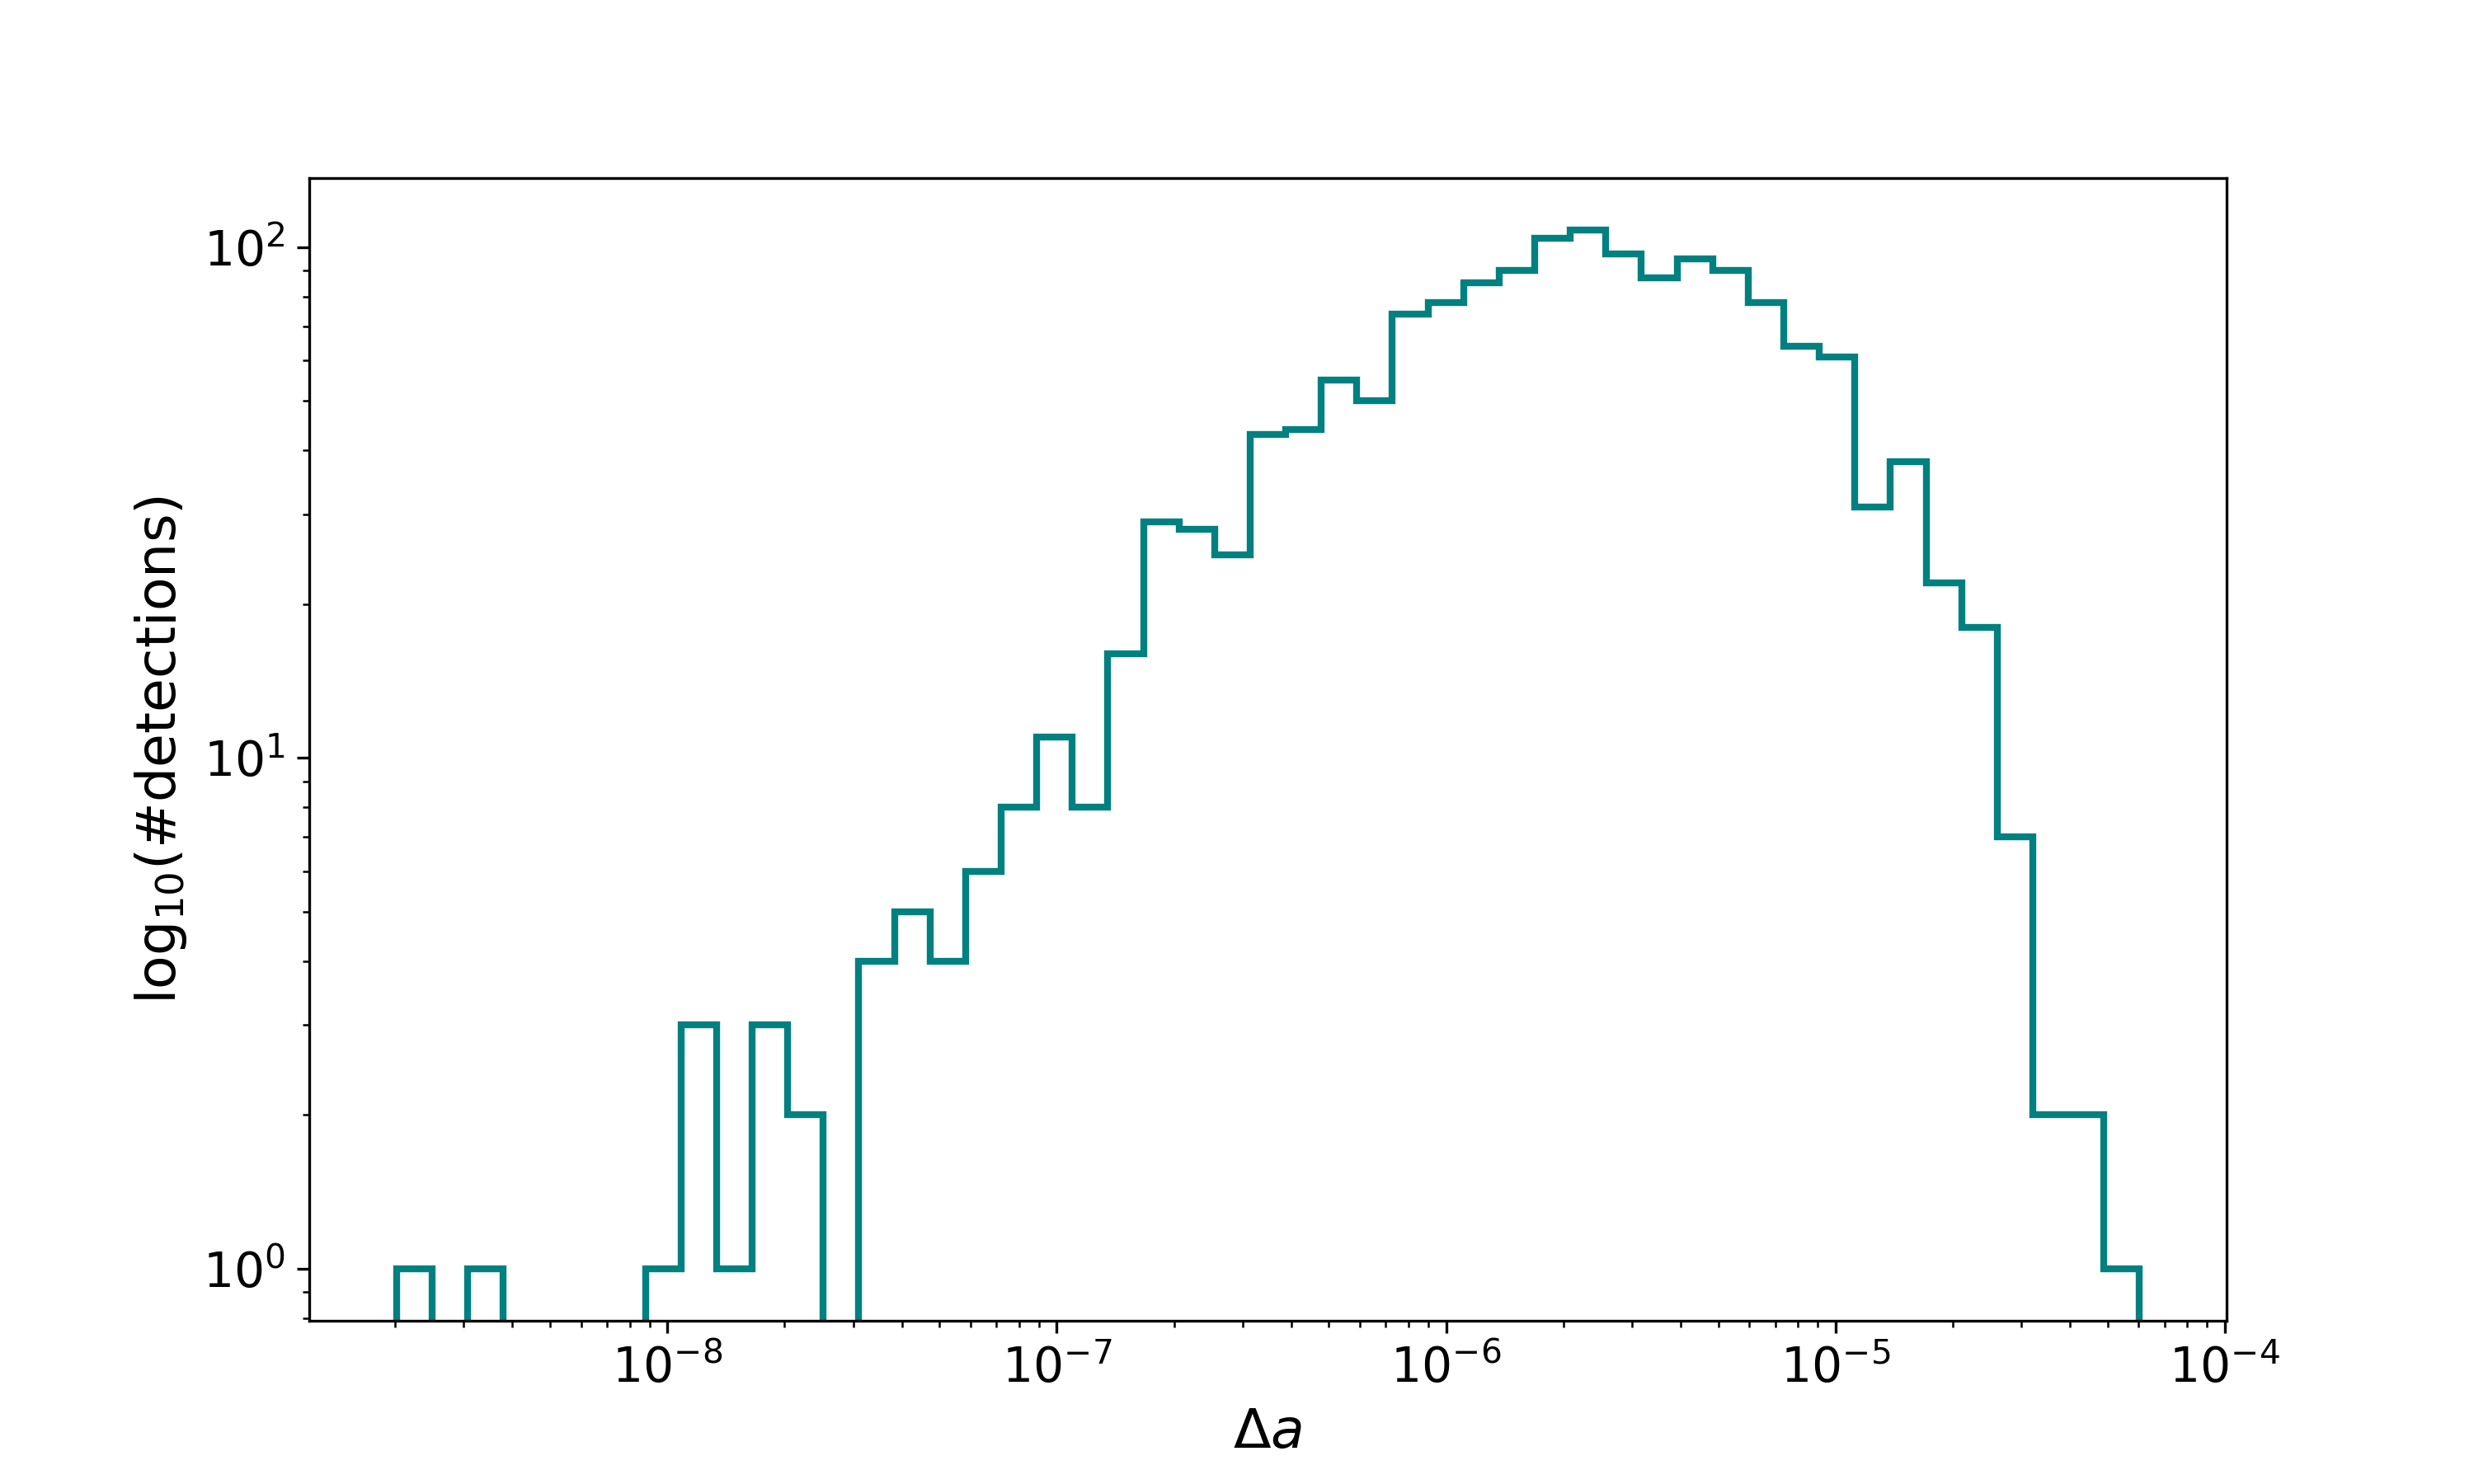
\includegraphics[width=0.49\textwidth]{parameter_estimation/a_uncertainties.png}
    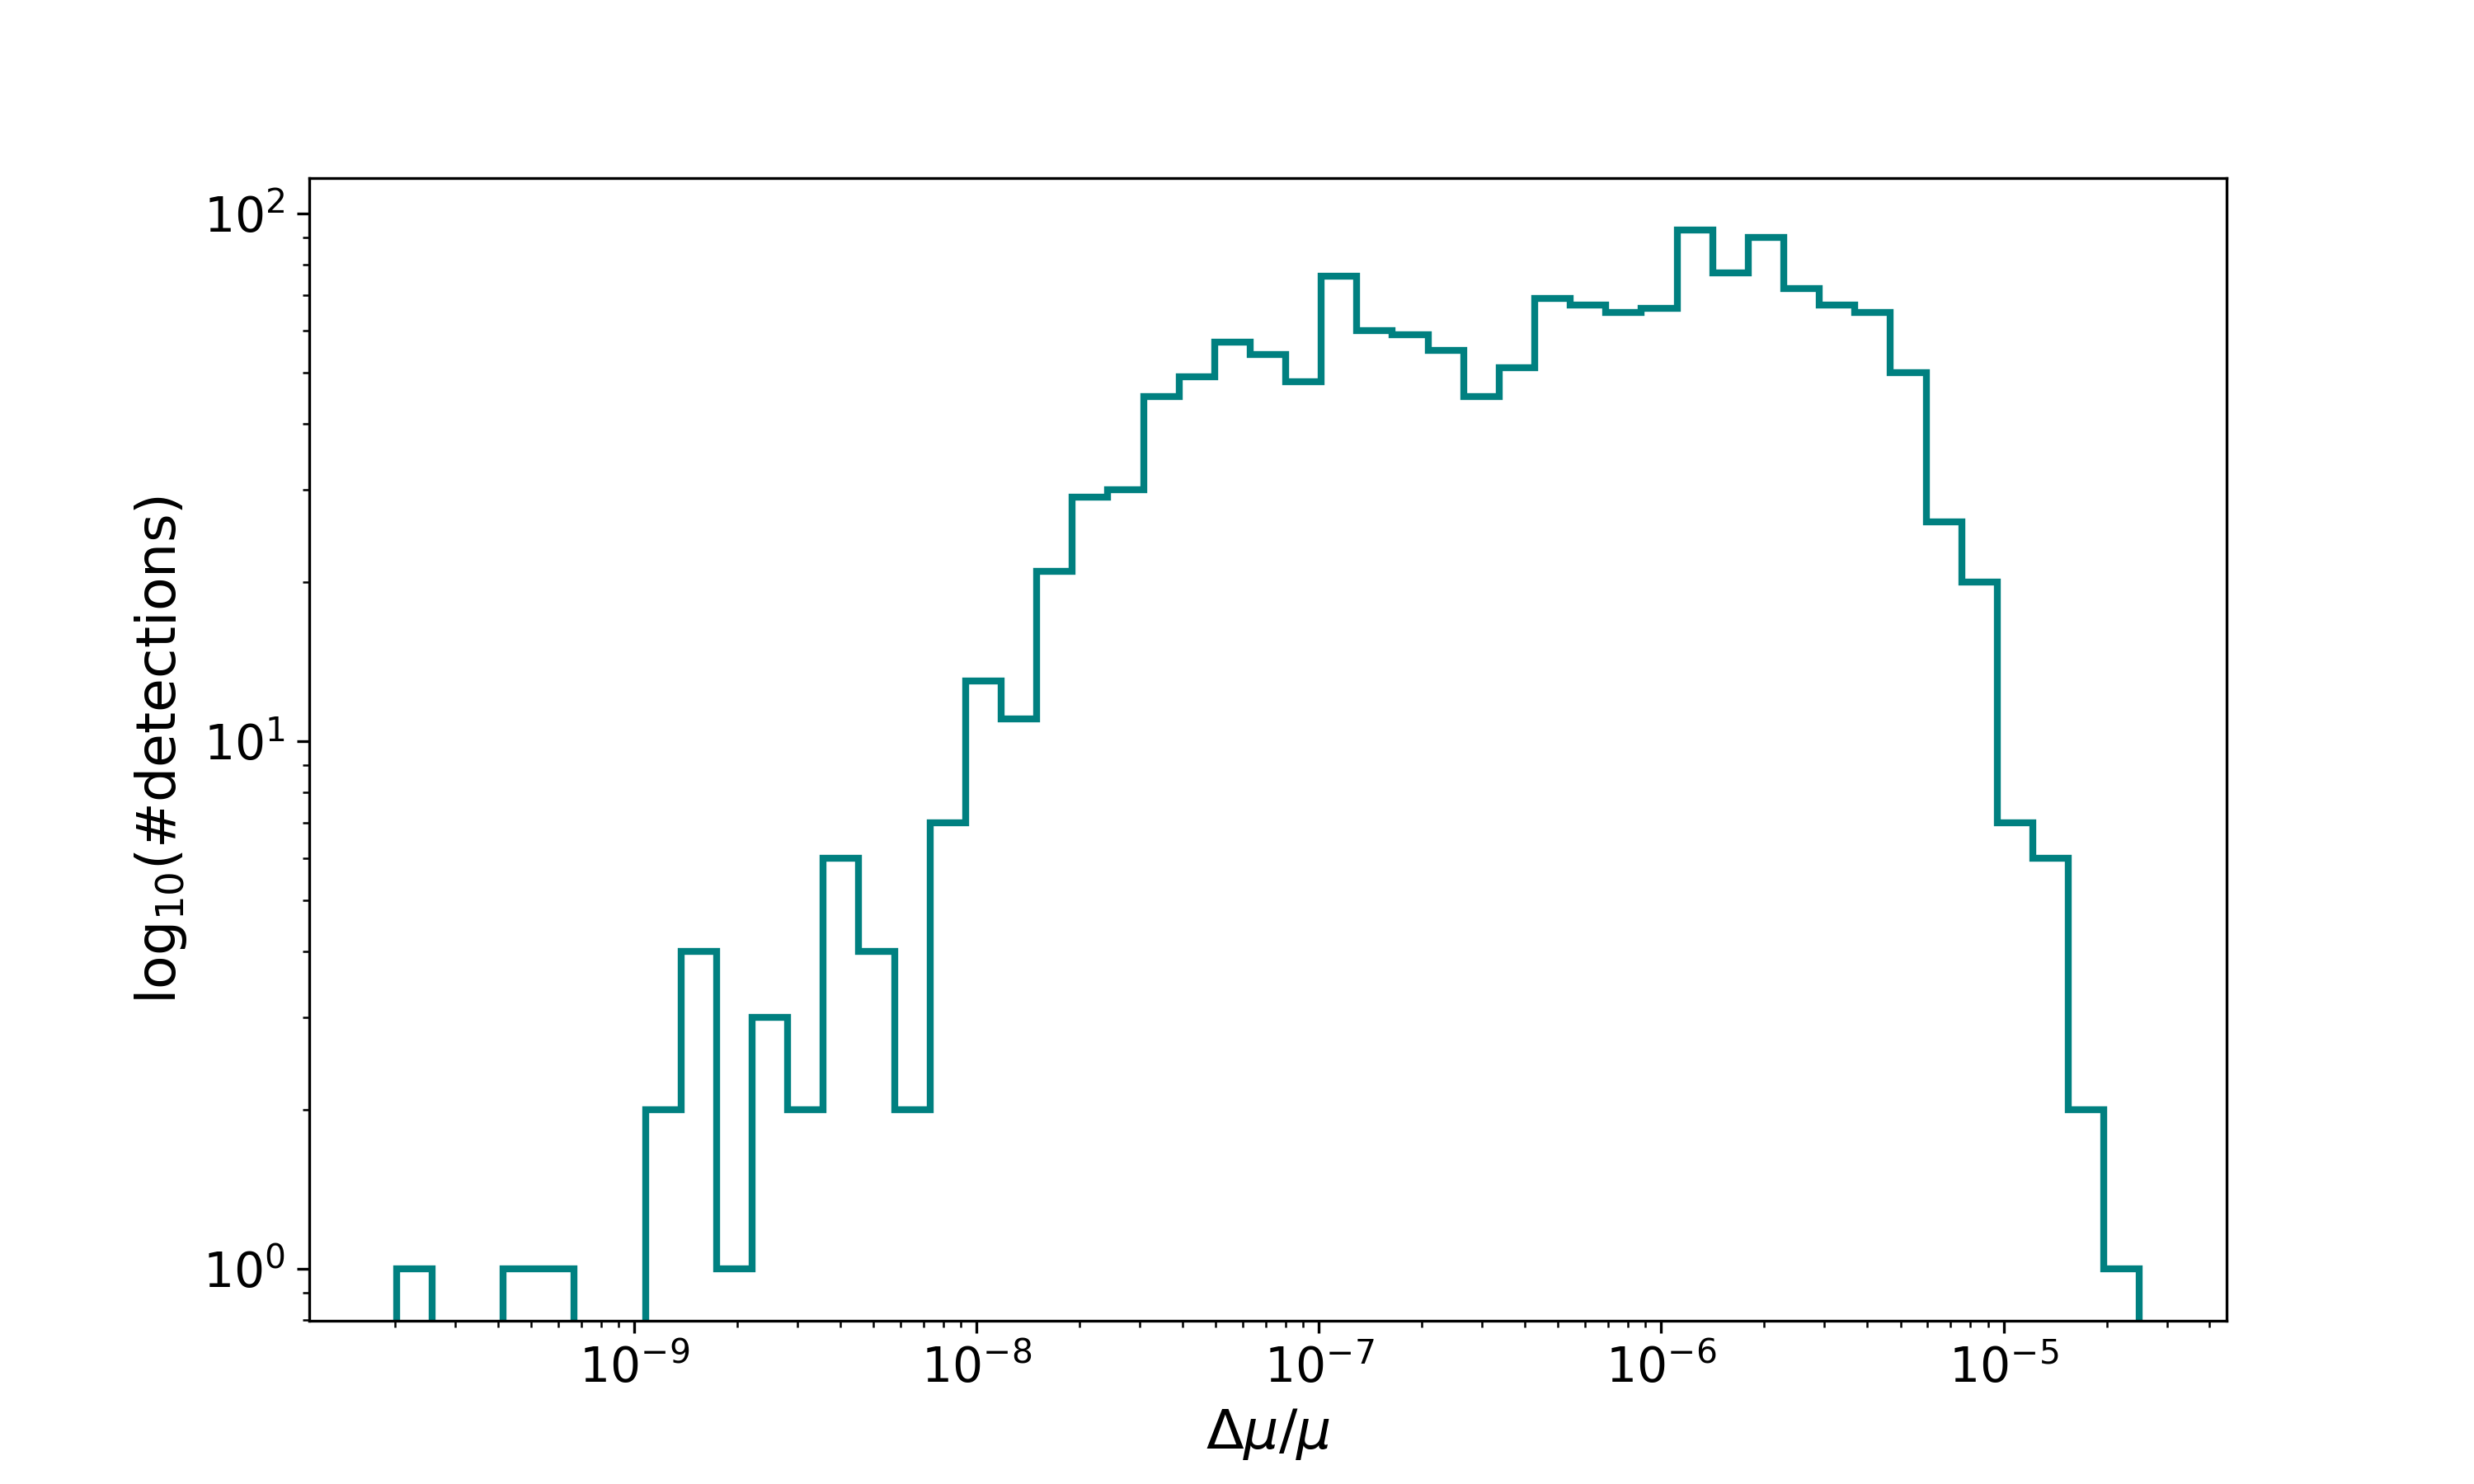
\includegraphics[width=0.49\textwidth]{parameter_estimation/mu_uncertainties.png}
    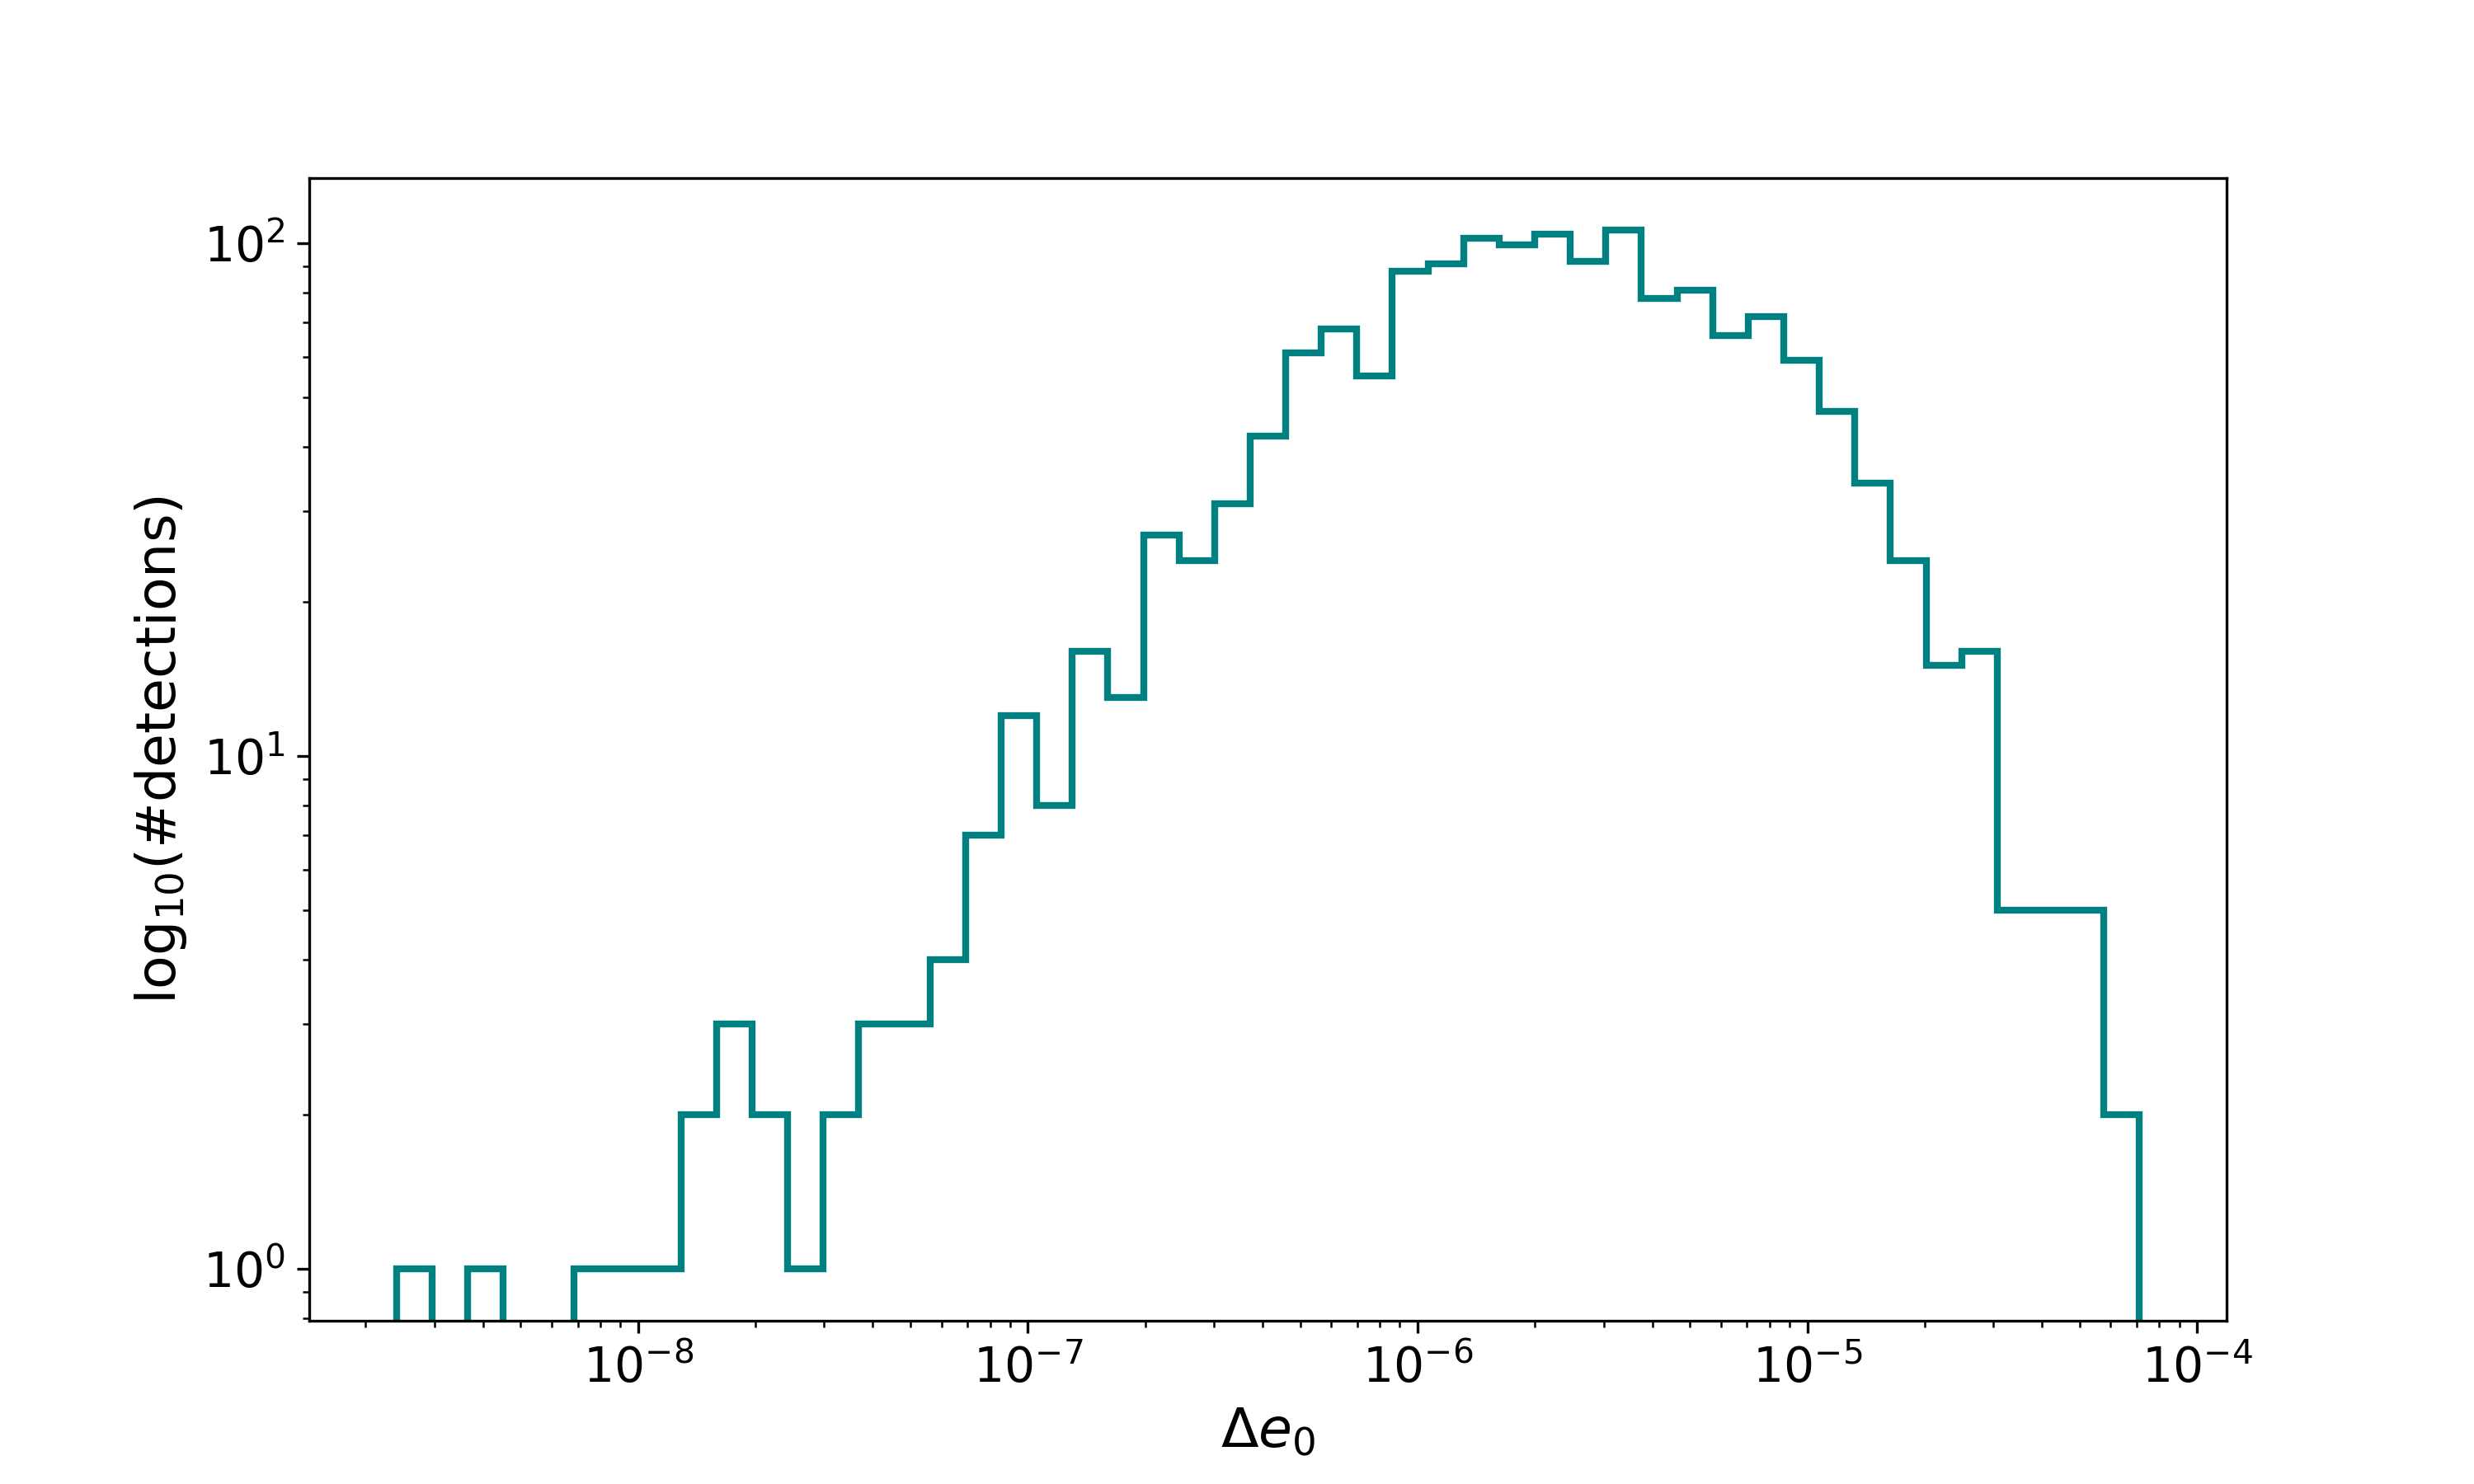
\includegraphics[width=0.49\textwidth]{parameter_estimation/e_uncertainties.png}
    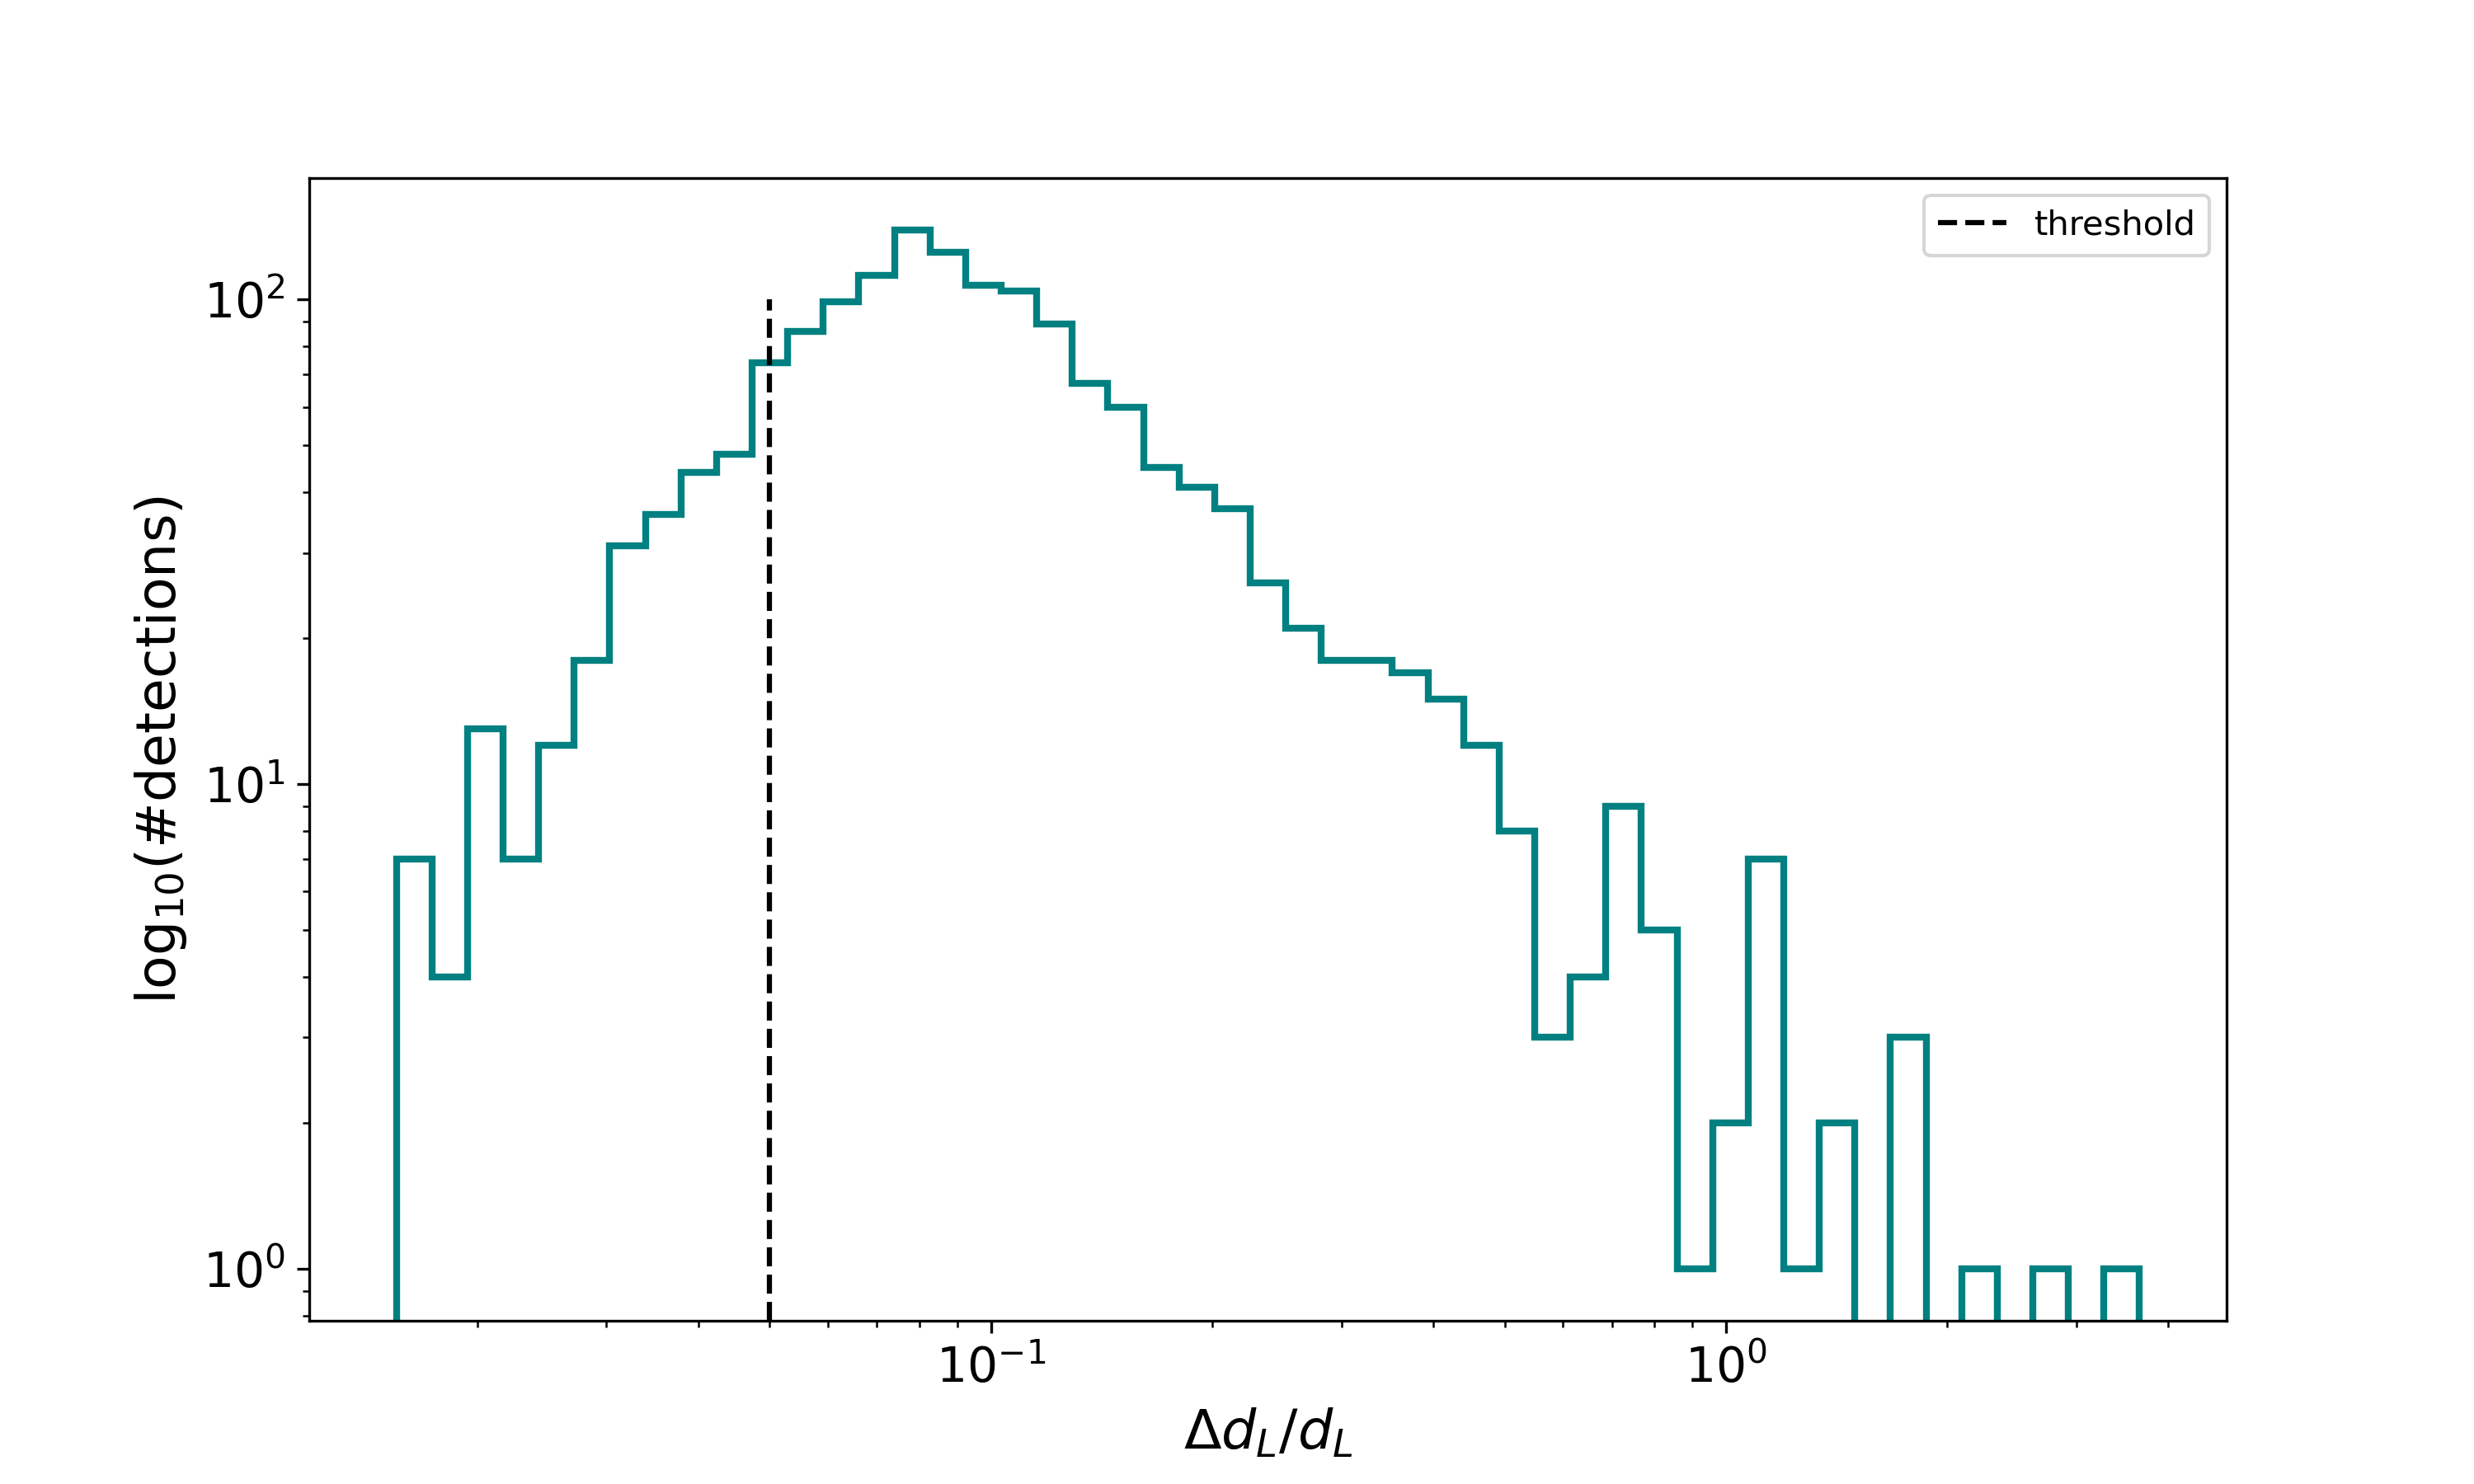
\includegraphics[width=0.49\textwidth]{parameter_estimation/dl_uncertainties.png}
    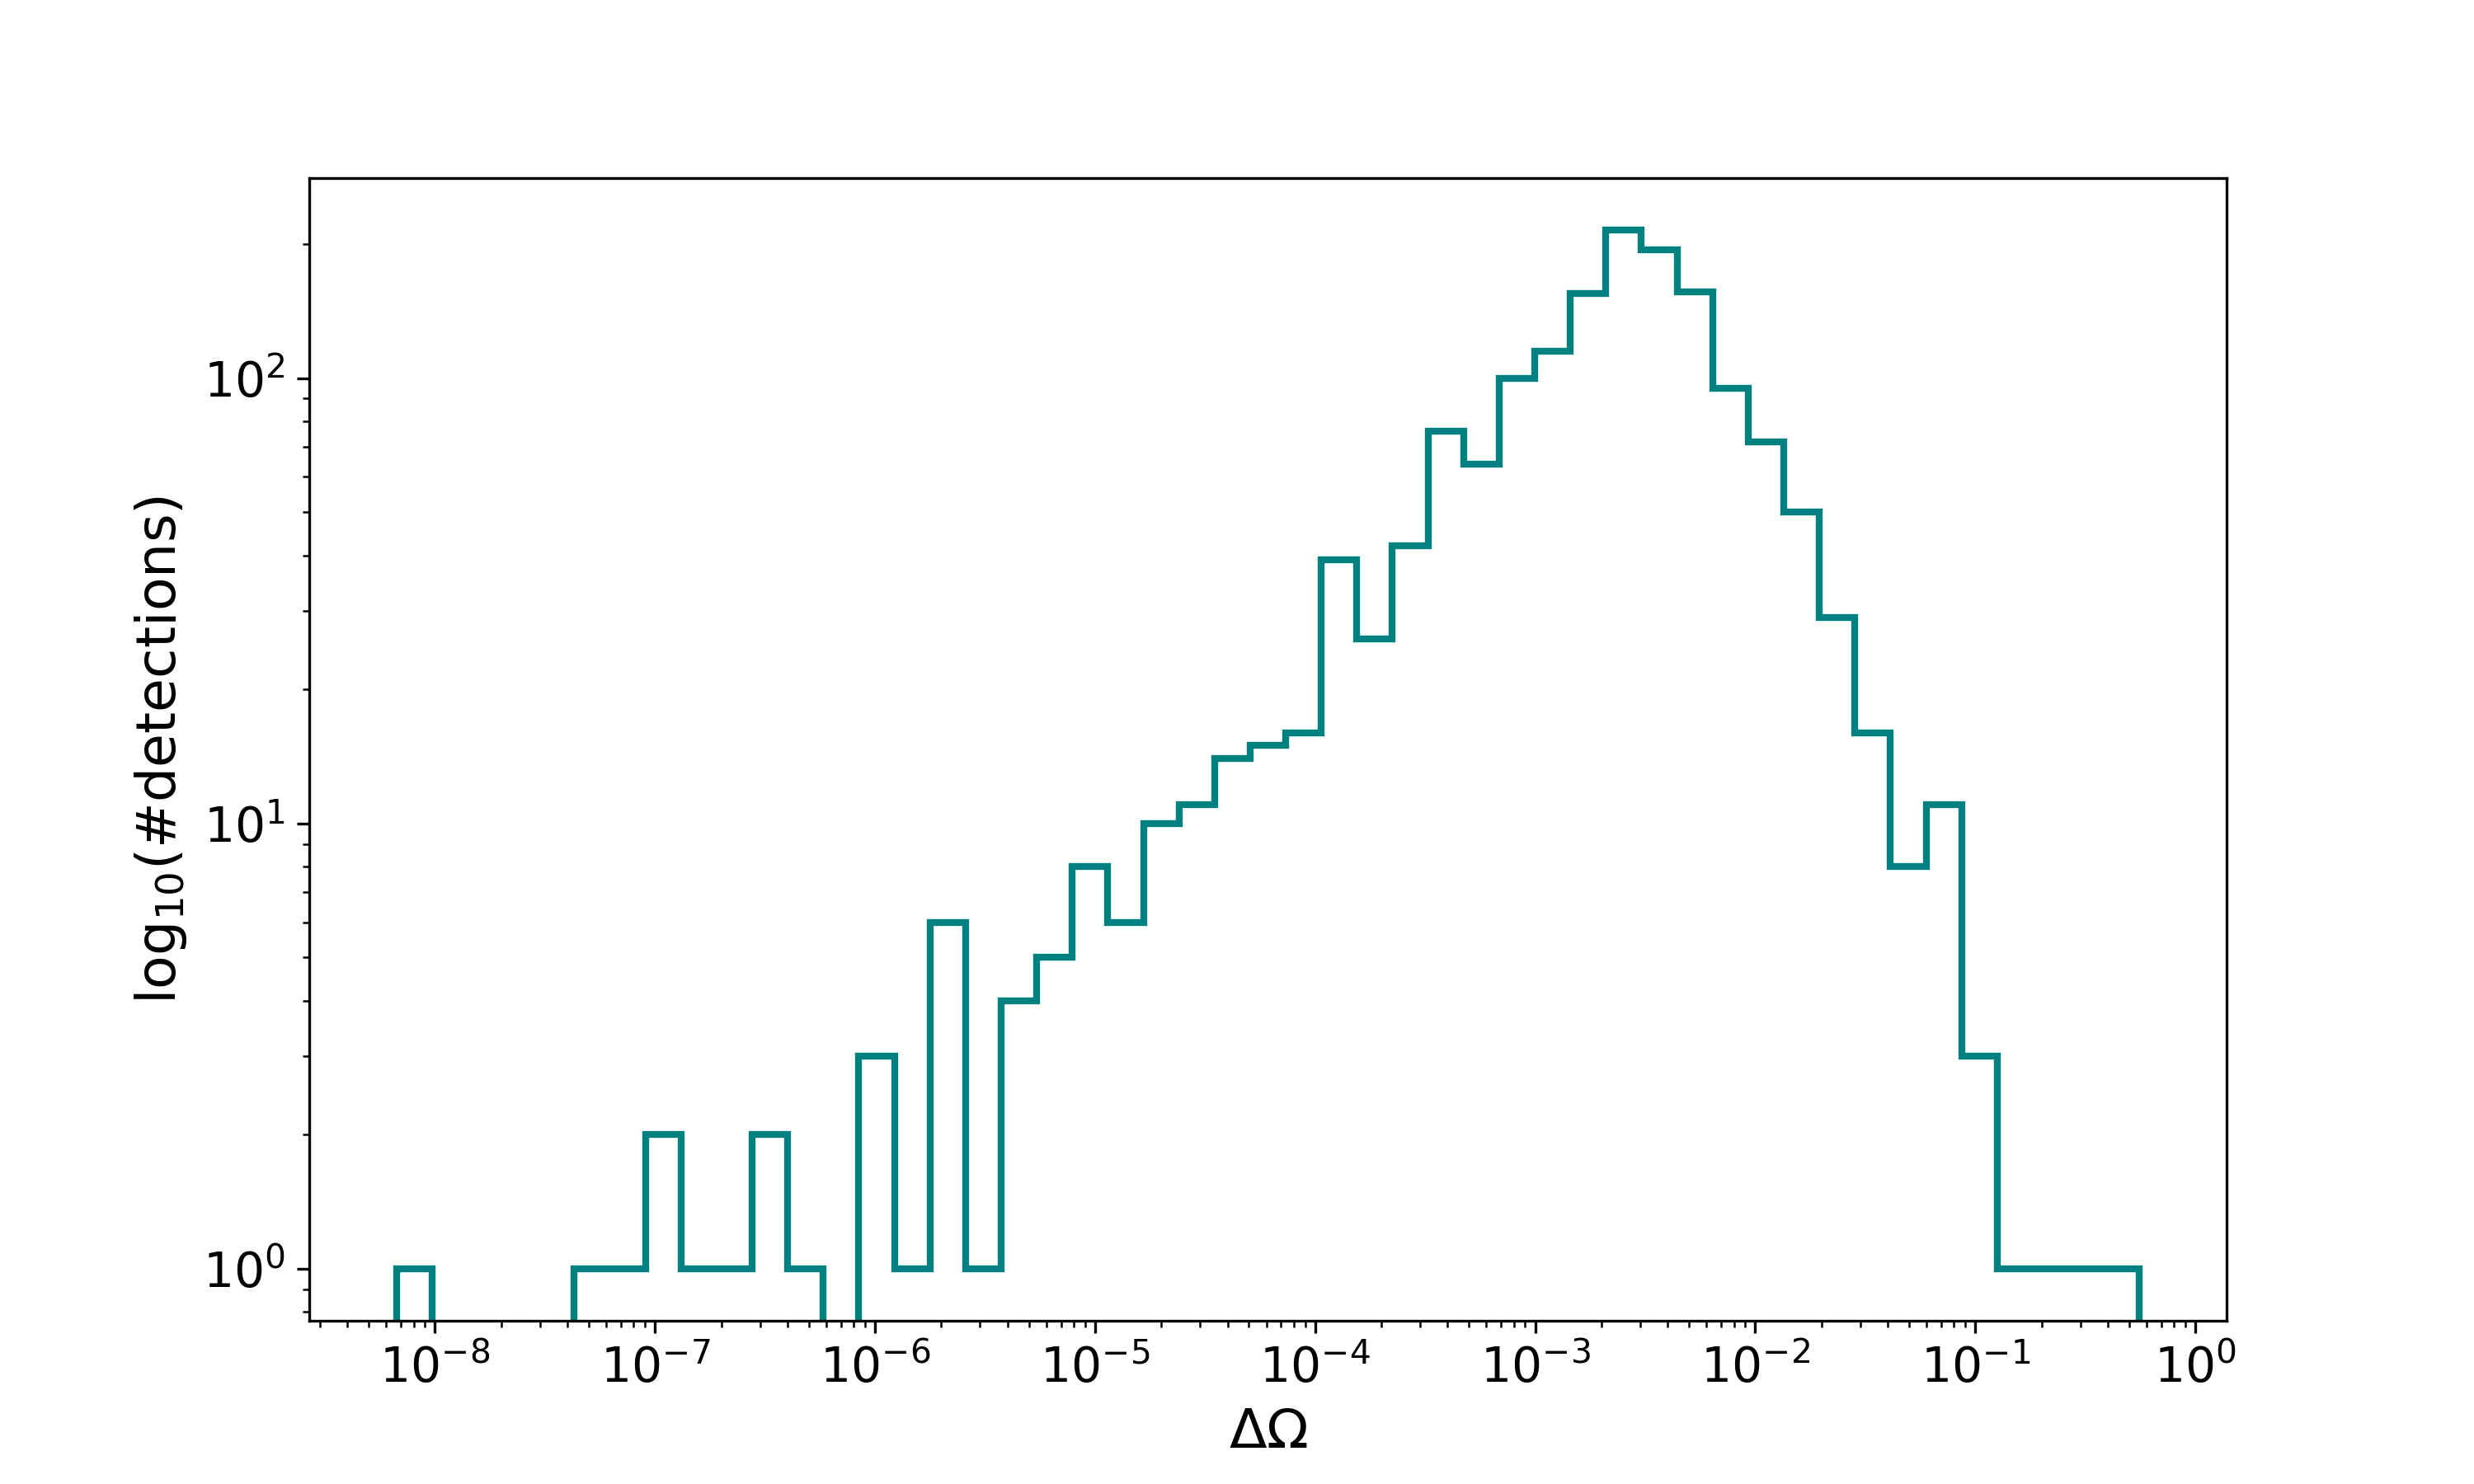
\includegraphics[width=0.49\textwidth]{parameter_estimation/omega_uncertainties.png}
    \caption[Parameter estimation results]{The results of the parameter estimation for all $N_\text{det}$ simulated detections. We show the errors on the measured parameters $\{ \Mz, \mu, \dl, e_0, a, (\vartheta, \varphi) \}$ with their $1-\sigma$ uncertainties.}
    \label{fig:parameter-estimation-results-galaxy-catalog-only}
\end{figure}

\section{Results for reduced Hubble constant constraints}\label{sec:results-for-reduced-hubble-constant-constraints}
In general, we will use the freedom of normalization in the posterior or for the likelihoods to normalize the posterior distributions to a maximum value of $1$.
\subsection{Normalization A}\label{subsec:galaxy-catalog-only-normalization-a}
For normalization A given in \fullref{eq:normalization-gair-23} we will directly show the posterior distribution of $\rhubble$ for subsets of 100 detections each in \fullref{fig:posteriors-normalization-a-subsets}. It is clear, that this inference method is strongly biased and does not yield any results. We can further illustrate the bias by showing the single event likelihoods in \fullref{fig:normalization-a-likelihoods}. In \cite[chapter 4.2]{Gair_2023} they talk about possible biases arising from inconsistencies in the inference. The two cases that would correspond to a strong bias to higher $\rhubble$ are the following:
\begin{enumerate}
    \item $z_\text{draw}$ is not accounted for in the inference. This means that we would only choose galaxies from a region, let us say $z<0.2$ but then also consider galaxies from larger redshifts. As we imposed $z_\text{draw} = 1.5$ which corresponds to all galaxies there are in the catalog for this region, this bias should not arise.
    \item GW detection probability: This refers exactly to the normalization that they introduce accounting for the GW detection probability. Potentially, it is incorrect to just choose the same threshold that they imposed in their work, as we clearly only draw events from lower redshifts and artificially have a lower threshold for the detection probability. This could be a possible explanation for the bias.
    \item The third possibility is, of course, that the normalization has been misunderstood or implemented incorrectly.
\end{enumerate}


\begin{figure}
    \centering
    \includegraphics[width=\textwidth]{normalization_a/bayesian_statistics_event_posteriors_subsets.png}
    \caption[Posterior distribution normalization A from subsets of the detections]{The posterior probability distribution of $\rhubble$ with normalization A \fullref{eq:normalization-gair-23} for subsets of 100 detections of the simulated detections with and without using the measured black hole mass $\Mz$. The vertical green dashed line indicates the true value of $\rhubbletrue = 0.73$.}
    \label{fig:posteriors-normalization-a-subsets}
\end{figure}

\begin{figure}
    \centering
    \includegraphics[width=0.49\textwidth]{normalization_a/bayesian_statistics_event_posteriors.png}
    \includegraphics[width=0.49\textwidth]{normalization_a/bayesian_statistics_event_posteriors_with_bh_mass.png}
    \caption[Single event likelihoods normalization A]{The likelihood of the single events for normalization A \fullref{eq:normalization-gair-23}, the product of which will give the posterior distribution for the simulated detections with and without using the measured black hole mass $\Mz$. Note that we have normalized the likelihoods to a maximum value of $1$ for better visibility. The vertical green dashed line indicates the true value of $\rhubbletrue = 0.73$.}
    \label{fig:normalization-a-likelihoods}
\end{figure}


\subsection{Normalization B}\label{subsec:galaxy-catalog-only-normalization-b}
In this scenario we used the normalization constant $\beta^\text{B}(\rhubble)$ defined in \fullref{eq:bias-correction-chen-22}. In \fullref{fig:posteriors-normalization-b} we show the posterior distribution $p(\rhubble| \detections, \galcat, \cosmologicalmodel, \backgroundinformation)$ using all $N_\text{det}^\text{posterior}$ detections. We can see that the posterior distribution maximizes close to $\rhubbletrue = 0.73$ and in the case of using the measured black hole mass $\Mz$ the posterior distribution is narrower and nearly follows a gaussian distribution. The results for the posterior without considering $\Mz$ we obtain one peak of the posterior very close to the true value and additionally a second peak shifted to lower values of $\rhubble$. Overall, we find the results
\begin{equation}
    \label{eq:results-normalization-b}
    \boxed{
        \begin{aligned}
            \bar{h}^\text{B}_\text{MBH} & = 0.7416 \pm 0.0132, \\
            \bar{h}^\text{B}            & = 0.7123 \pm 0.0283,
        \end{aligned}
    }
\end{equation}
when fitting a gaussian distribution to the posterior distribution. This corresponds to an accuracy of the measurements of
\begin{equation}
    \label{eq:results-normalization-b-relative-error}
    \boxed{
        \begin{aligned}
            \frac{\Delta h^\text{B}_\text{MBH}}{\bar{h}^\text{B}_\text{MBH}} & \approx 1.8\%, \\
            \frac{\Delta h^\text{B}_\text{MBH}}{\bar{h}^\text{B}_\text{MBH}} & \approx 4\%,
        \end{aligned}
    }
\end{equation}
and relative mean deviation from the true value $\rhubbletrue$
\begin{equation}
    \label{eq:results-normalization-b-relative-deviation}
    \boxed{
        \begin{aligned}
            \frac{\bar{h}^\text{B}_\text{MBH} - \rhubbletrue}{\rhubbletrue} & \approx 1.6\%,  \\
            \frac{\bar{h}^\text{B} - \rhubbletrue}{\rhubbletrue}            & \approx -2.4\%.
        \end{aligned}
    }
\end{equation}
To see the biases in the posterior distribution we show the posterior distribution for randomly chosen subsets of 100 detections each in \fullref{fig:posteriors-normalization-b-subsets}. We can clearly see that in the case without the MBH mass the posterior distribution often increases towards the bounds of the prior range of $\rhubble$ while for the evaluation with the MBH mass the posterior looks overall better and behaves well towards the bounds of the range of $\rhubble$ but the mean value or the sigma deviation is always shifted higher values of $\rhubble$ which also corresponds to a bias. To have a comparison to the clear bias in the case of normalization A, we also plot the single event likelihood in \fullref{fig:normalization-b-likelihoods}. Here it is visible that the uninformative detections are just close to being flat instead of increasing towards higher values of $\rhubble$.


\begin{figure}
    \centering
    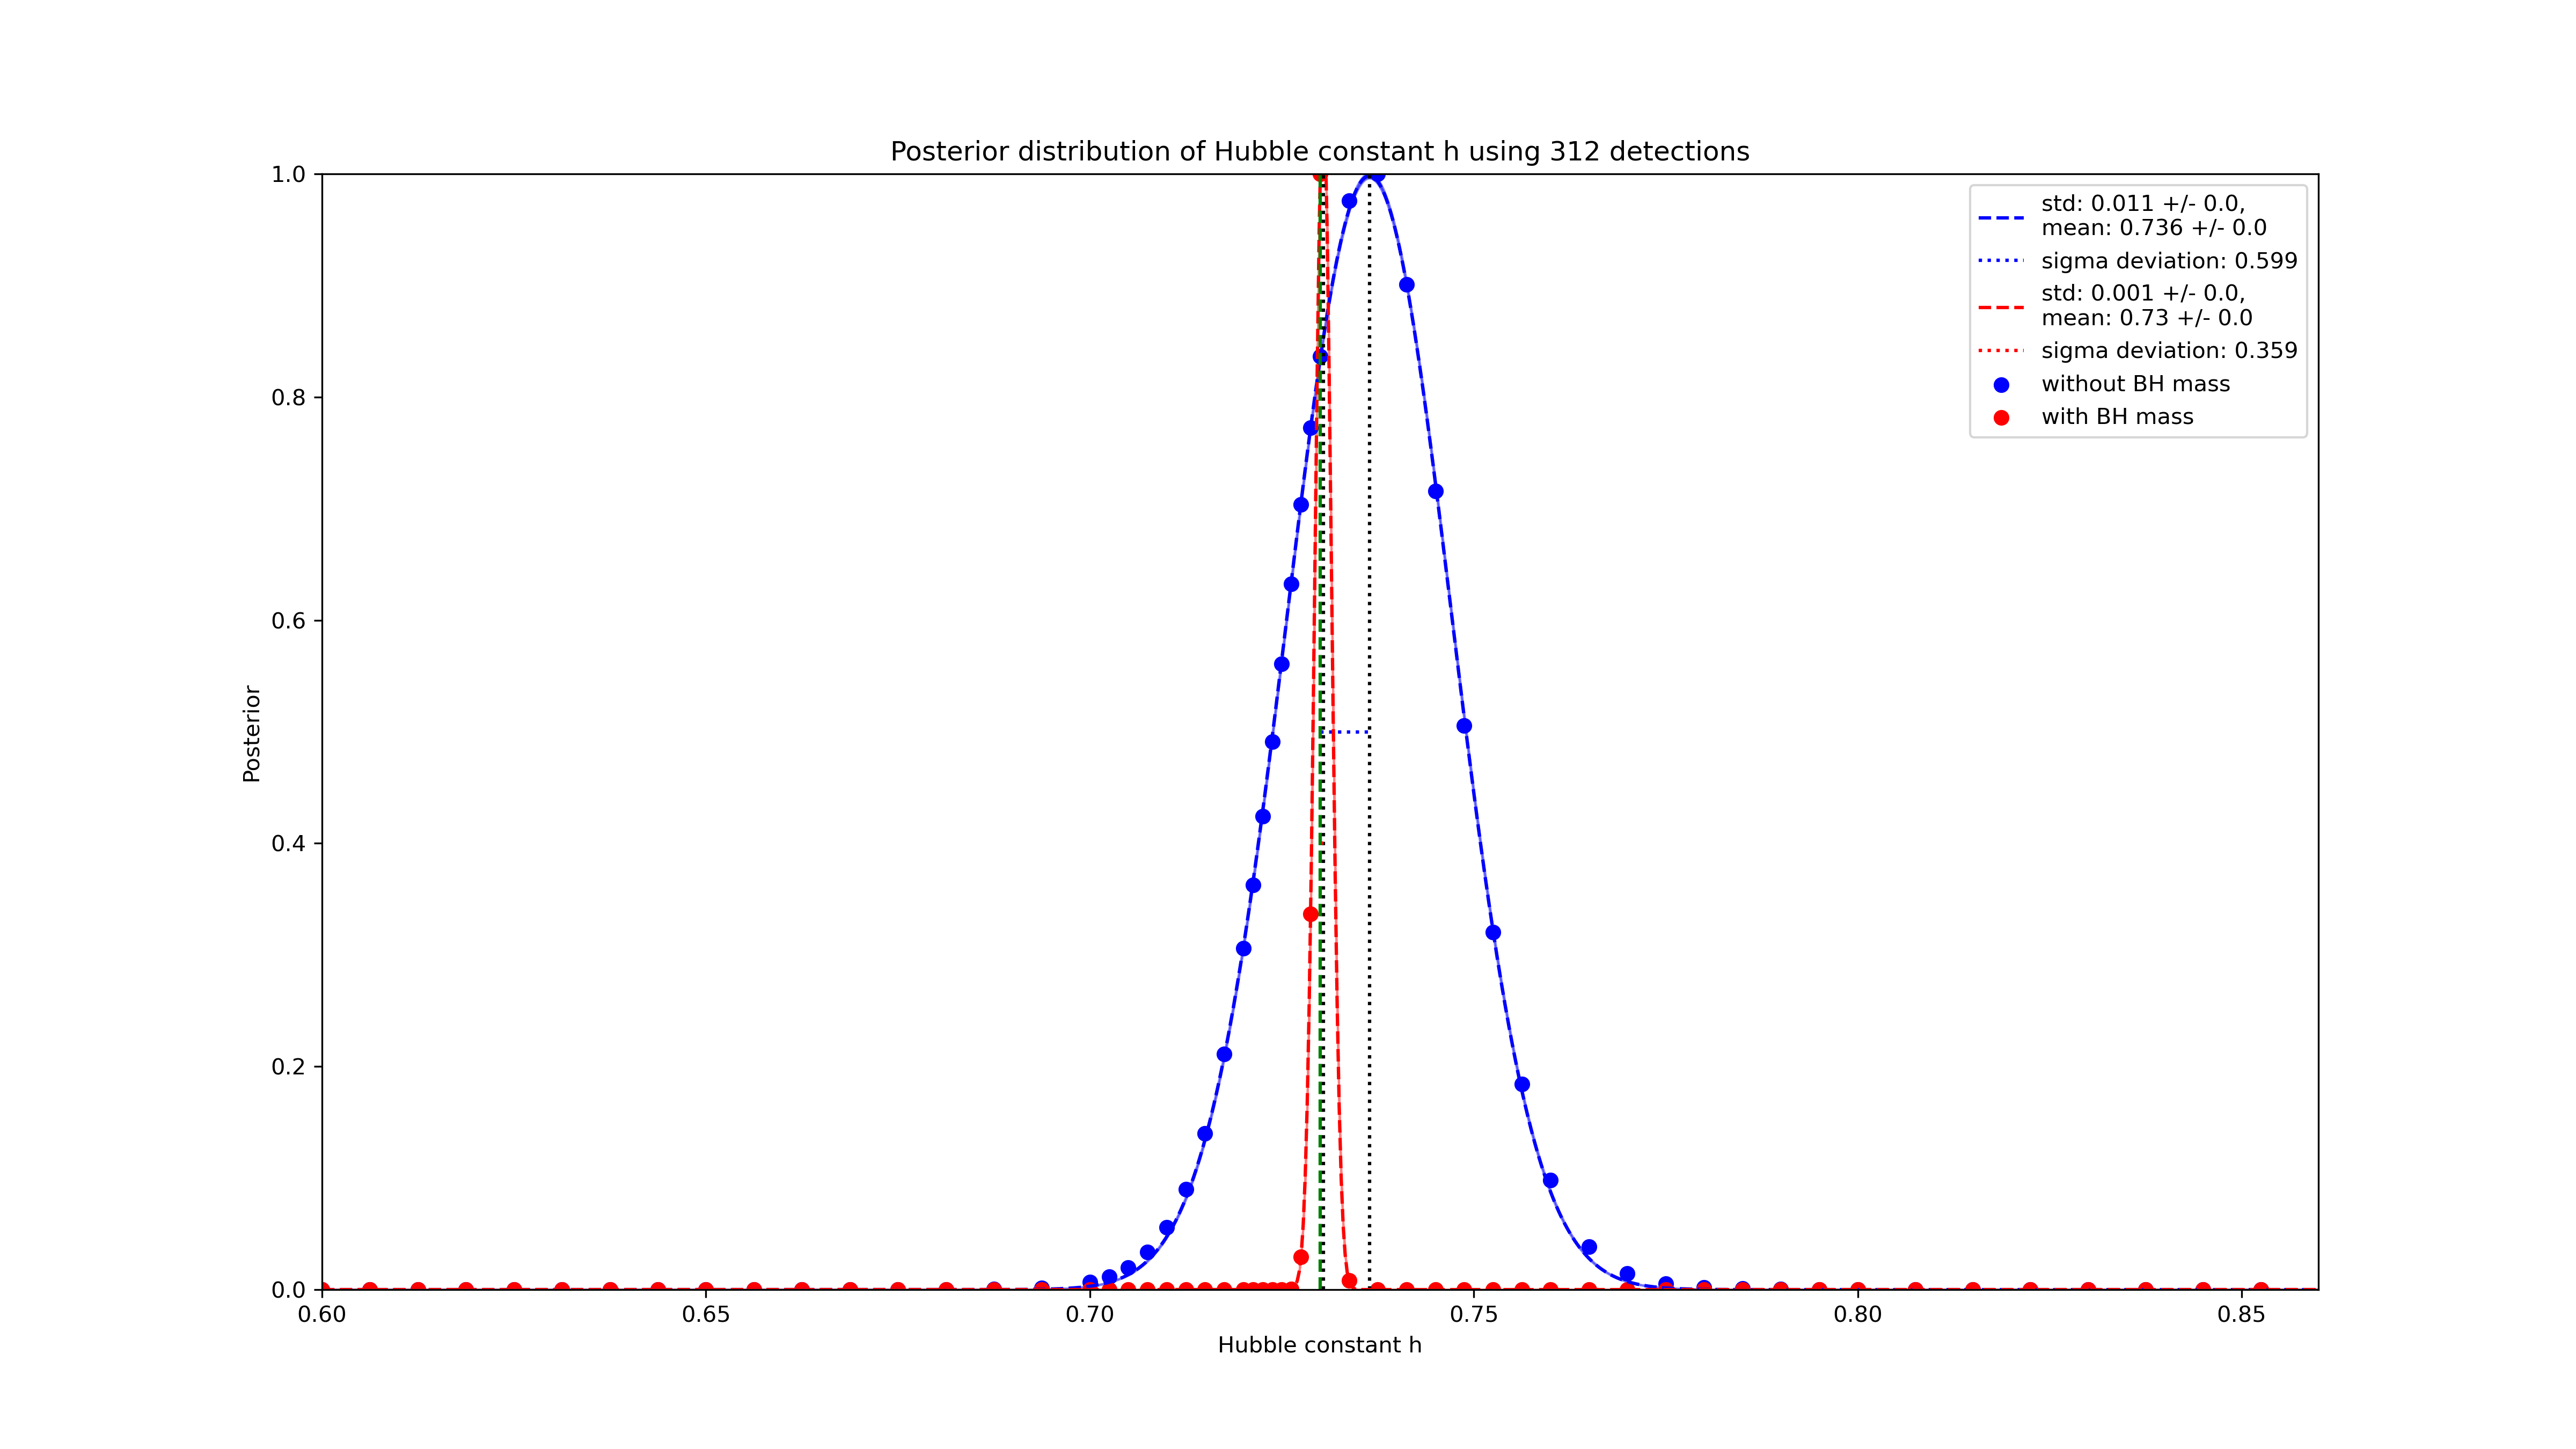
\includegraphics[width=\textwidth]{normalization_b/bayesian_statistics.png}
    \caption[Posterior distribution normalization B]{The posterior probability distribution of $\rhubble$ with normalization B \fullref{eq:bias-correction-chen-22} for the simulated detections with and without using the measured black hole mass $\Mz$. The vertical green dashed line indicates the true value of $\rhubbletrue = 0.73$.}
    \label{fig:posteriors-normalization-b}
\end{figure}

\begin{figure}
    \centering
    \includegraphics[width=\textwidth]{normalization_b/bayesian_statistics_event_posteriors_subsets.png}
    \caption[Posterior distribution normalization B subsets]{The posterior probability distribution of $\rhubble$ with normalization B \fullref{eq:bias-correction-chen-22} for randomly chosen subsets of simulated detections with and without using the measured black hole mass $\Mz$. The vertical green dashed line indicates the true value of $\rhubbletrue = 0.73$.}
    \label{fig:posteriors-normalization-b-subsets}
\end{figure}

\begin{figure}
    \centering
    \includegraphics[width=0.49\textwidth]{normalization_b/bayesian_statistics_event_posteriors.png}
    \includegraphics[width=0.49\textwidth]{normalization_b/bayesian_statistics_event_posteriors_with_bh_mass.png}
    \caption[Single event likelihoods normalization B]{The likelihood of the single events for normalization B \fullref{eq:bias-correction-chen-22}, the product of which will give the posterior distribution for the simulated detections with and without using the measured black hole mass $\Mz$. Note that we have normalized the likelihoods to a maximum value of $1$ for better visibility. The vertical green dashed line indicates the true value of $\rhubbletrue = 0.73$.}
    \label{fig:normalization-b-likelihoods}
\end{figure}